\chapter{Project Plan}
	
\section{Planning}
	Much of the planning was facilitated by our weekly meetings with David Watkins, our TA. He very clearly explained what the requirements of each milestone entailed, and helped keep expectations transparent. Since Professor Edwards had emphasized the need for vertical development of features instead of horizontal building of each compiler layer, we quickly identified the key features that would be required to enable the key functionality of our language. Two of the most important components were structs and threads.

  \medskip \noindent
  Our initial plan, which we largely followed, was to complete the Language Reference Manual, experiment with the layers of the compiler and get \texttt{Hello, World!} working, and then use what we had learned to begin implementing the more crucial aspects of the language.

\section{Workflow}
 
  \begin{center}
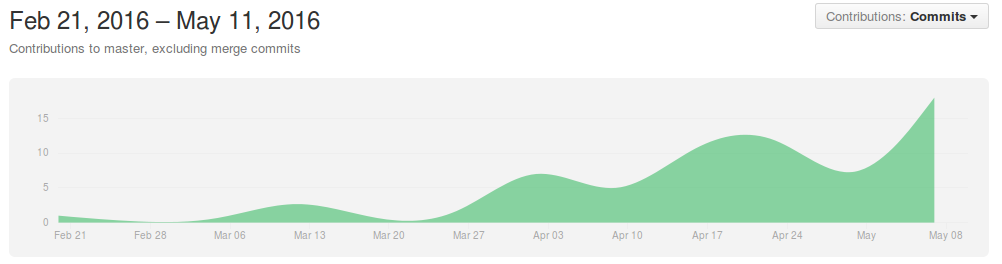
\includegraphics[width=.9\textwidth]{img/gitlog_graph.png}
  \end{center}
  Workflow was facilitated by Git and GitHub, which allowed for the team to easily work on multiple features simultaneously and (usually) merge together features without overlapping conflicts. The Git workflow reached an optimal point by the conclusion of the project; new features would be developed, tested, and finalized in separate branches, and the commits for that feature would be squashed down until a single commit representing the new feature would be merged into the master branch.

  \medskip \noindent
  Features were developed individually or through paired programming, depending on the scope and complexity of the feature. GitHub and division of labor allowed for many team members to work independently, at different times of the day per their own schedule. Branching allowed for one person to quickly deploy buggy code to another in hopes of resolving the issue, without any modification or bad commits to the master branch. GroupMe was used extensively for inter-team communication.

\section{Team Member Responsibilities}
  

  \begin{tabular}{ | l | l | l |}\hline
    Team Member  & Responsibilities      & GitHub Handle\\ \hline
    Amy Xu & structs, nested structs, pointers, malloc & axxu\\
    Emily Pakulski & C-bindings, reformatting tests, atomicity & ohEmily\\
    Amarto Rajaram & C-bindings, pthread, file I/O, malloc & Amarto\\
    Kyle Lee & structs, LRM, Final Report, debug and assist Amy & kyle--lee\\ \hline
  \end{tabular}
\newpage
\section{Git Logs}

Note that `PLT Student' was team member Amy Xu.
    
\subsection{master branch}

    \begin{lstlisting}[backgroundcolor=\color{white}]
commit 4ecbc629057cc19c839d5e0f5f9224b88710ac8e
Merge: d0a23f0 cb6b509
Author: Amy Xin Xu <axxu3795@gmail.com>
Date:   Wed May 11 18:04:44 2016 -0400

    Merge pull request #24 from DemocritusLang/linkedlist_and_stack
    
    Final linked list demo

commit cb6b5091e6812c3f3a60869bdb39bdd6900c201e
Author: PLT Student <axxu3795@gmail.com>
Date:   Wed May 11 17:35:32 2016 -0400

    Final linked list demo
    
    Fixed merge accident
    
    Fixed malloc size
    
    Added to demo folder

commit d0a23f079f4a9828c6d2724141c5b7de1a126958
Author: Emily Pakulski <enp2111@columbia.edu>
Date:   Wed May 11 17:52:08 2016 -0400

    Added simple threads test.

commit e113aa58cc30af12cad615d07ed57b99905e0edf
Author: Emily <ohEmily@users.noreply.github.com>
Date:   Wed May 11 16:26:44 2016 -0400

    Multithreading and networking working together. Added concurrent comic download. (#23)
    
    * Added multithreaded test- getting parse error. Added strcat and int to string wrappers
    
    * fixed parse error.
    
    * Added memset to fix test-multithreaded-sockets.
    
    * Fix memset bug
    
    * Updated test file so sockets test passes
    
    * Fixed thread function signature
    
    * Added failing test.
    
    * Fixed bug in init_thread() and added test that passes string into thread().
    
    * possibly fixed request bug.
    
    * Fixed binary file reading bugs.
    
    * Moved code into demo directory.
    
    * Fixed merge conflicts after rebase.

commit d4972e0ff8b5ba850bf39528cc0b113bc1912ee5
Merge: dbb06cc 232be1f
Author: Amy Xin Xu <axxu3795@gmail.com>
Date:   Wed May 11 16:10:39 2016 -0400

    Merge pull request #22 from DemocritusLang/build_malloc_attempt
    
    Malloc and simple linked lists working

commit 232be1f27fb7ffa7110e5184c6016b81e2da94ff
Author: PLT Student <axxu3795@gmail.com>
Date:   Wed May 11 03:45:50 2016 -0400

    Malloc and simple linked lists working
    
    Fixed shift reduce errors
    
    temp commit
    
    CASTING AND MALLOC WORK
    
    Cleaned up warnings
    
    Cleaned up codegen warnings
    
    Fixed (*a). dotops and halfassed addnode
    
    Half way linked lists
    
    Linked lists with add and print_list functions

commit dbb06cc9f0f2f608583946158d48d8d841d8dc62
Author: Emily Pakulski <enp2111@columbia.edu>
Date:   Wed May 11 13:30:05 2016 -0400

    Added check in tester for whether code was already compiled.

commit 36aee48817bdeec1553b1c16963e5abcc7aaaa6b
Merge: 0371f67 2402f74
Author: Amarto <aar2160@columbia.edu>
Date:   Wed May 11 06:10:49 2016 -0400

    Merge pull request #21 from DemocritusLang/sockets_finished
    
    Sockets finished

commit 2402f740bec59d6ed4912b2ee302d9b9b7bb5480
Author: Amarto <aar2160@columbia.edu>
Date:   Wed May 11 05:45:05 2016 -0400

    Added free(), execl wrapper, and corrected output reference for socket test. Changed tests to use free() after malloc. Refactored the weblink downloading method to only take one param so it matches the signature for a thread function

commit 170645297d4578f9551f690b08b82718beebf033
Author: Emily Pakulski <enp2111@columbia.edu>
Date:   Wed May 11 01:44:23 2016 -0400

    Changed up get request impl a bit.

commit 5226ad21d850b6622e09388a4337d0b515123f76
Author: Amarto <aar2160@columbia.edu>
Date:   Tue May 10 17:46:11 2016 -0400

    Added basic socket impl and loading files. Need to handle tests

commit 0371f67bac394c08ae72cb372491fd3264839f65
Merge: a6ce096 a784099
Author: Amy Xin Xu <axxu3795@gmail.com>
Date:   Wed May 11 02:57:57 2016 -0400

    Merge pull request #20 from DemocritusLang/add_float_and_mod
    
    Added modulo and floats

commit a78409901632a6f70e889fee8f5ccff2bfe12989
Author: PLT Student <axxu3795@gmail.com>
Date:   Tue May 10 23:26:55 2016 -0400

    Added modulo and floats
    
    Mod done
    
    Working on floats
    
    fixed floating print issue
    
    Working floats
    
    Added floats in struct test

commit a6ce096863beb92e5b5251b0802613edab31cc76
Author: Emily <ohEmily@users.noreply.github.com>
Date:   Tue May 10 23:09:23 2016 -0400

    Added sleep function and test. (#18)

commit ff330840be2c13aeed6f2a6d87a69ce153f29421
Merge: a63b40f fdcadf4
Author: Amy Xin Xu <axxu3795@gmail.com>
Date:   Tue May 10 15:28:57 2016 -0400

    Merge pull request #17 from DemocritusLang/add_pointers
    
    Pointers done

commit fdcadf4fa032354c8a9ec96f41cecb76b94e66f0
Author: PLT Student <axxu3795@gmail.com>
Date:   Tue May 10 02:02:43 2016 -0400

    Pointers done
    
    Dereference syntax there, need to clean warning
    
    Added ref op and semantic checking
    
    Working pointers for ints, need to test rest
    
    Modified test-pointer-int.dem for clarity and wrote test-pointer-bool, passing
    
    Added single and multilevel struct tests, passing
    
    Linkedlist test not working
    
    Added hypothetical linkedlist tests (not working
    
    Linked of list proof of concept
    
    Changed type* to *type to reflect Go syntax

commit a63b40fb618149ec65e57ea3ac986bdccf9f4ac4
Author: Kyle Lee <kylelee.contact@gmail.com>
Date:   Tue May 10 01:11:44 2016 -0400

    Added singleline comments

commit 901814668aa2d7513fe74b45fa4390d82635ac01
Author: Amarto <aar2160@columbia.edu>
Date:   Tue May 10 00:46:58 2016 -0400

    Fixed void pointer notation to match Go syntax, fixed test

commit 0ed94930f8362cb6eb322ec6a9570043660aabb5
Merge: b662f67 d9b467b
Author: Amy Xin Xu <axxu3795@gmail.com>
Date:   Tue May 10 00:43:18 2016 -0400

    Merge pull request #15 from DemocritusLang/clean_nested_structs
    
    Working nested structs

commit d9b467b80ce152696875d6ec1d3d2f1ec6ea77e6
Author: PLT Student <axxu3795@gmail.com>
Date:   Mon May 9 22:47:07 2016 -0400

    Working nested structs
    
    Added nested struct test
    
    Fixed mistyped identifier
    
    nested structs working
    
    Fixed typo in test-structs-nested.out and added another test
    
    Edited test to be more informative of functionality
    
    test-struct-nested1

commit b662f676ae12fbb27eedaf5af6ae990d76f423bc
Author: Emily Pakulski <enp2111@columbia.edu>
Date:   Mon May 9 20:34:05 2016 -0400

    Finished file I/O. lseek also implemented.

commit 84c1fc11bc2a2e59b8fec9d68937db8205f1b5d9
Author: Amarto <aar2160@columbia.edu>
Date:   Sun May 8 20:30:58 2016 -0400

    Added malloc and started file I/O.

commit 8b3944051cfde07be958214aae56bf47988fb803
Author: Emily <ohEmily@users.noreply.github.com>
Date:   Mon May 9 11:15:23 2016 -0400

    Updated all instances of MicroC to Democritus and added 'make all' target (#12)
    
    * Changed MicroC -> Democritus and added make all target.
    
    * Changed file extension for democrituslang files from .mc to .dem.

commit ed27ce5f8a31a740f3eb0e5ad3ff3cfcf7a838f9
Author: Amarto <aar2160@columbia.edu>
Date:   Sun May 8 19:31:43 2016 -0400

    Fixed warnings resulting from merge

commit c6cbdf15fd8854a02fb695fa9aa41b50966431a7
Author: Amarto <aar2160@columbia.edu>
Date:   Sat Apr 30 15:16:57 2016 -0400

    Added multithreading and void pointers, and added calling bound C functions
    Added declaration of thread() function to codegen. Everything compiles
    
    Added basic threads checking to semant.ml. Need to wait until arguments for pthread are passed in
    
    Working on codegen.ml, but getting compiler warning. Working on threading test, but need NULL keyword?
    
    Added tests for threading and modified codegen and semant
    
    Baby steps. Still not working. (temp commit).
    
    Oops. But still not working.
    
    Fixed some things in test case. Pretty sure function name should be passed in as a string. (temp commit.)
    
    Temp commit. More debug info. Maybe fixed some bugs but same error.
    
    temp commit - fixed compiler warning but old tests are failing
    
    Fixed old tests, fixed compiler warning
    
    Added correct(?) invocation of args in thread_init. Still not_found exception
    
    It was failing to match on [e]. Changed to e, and now it's giving a broken module error: params don't match
    
    Still not working (broken module) but now using lookup_function and pattern matching to remove option
    
    Added a void ptr type for thread (kinda hacky for now but it's for testing threads). Also it's now finding the function from the string name
    
    Added thread testing script
    
    THREADS NOW WORK IN SCRIPT!!!
    
    Passing threading test
    
    Fixed compiler warnings from pattern matching in codegen

commit bca9388f1d5b7011fde7461b2f1055562f1c7561
Author: PLT Student <axxu3795@gmail.com>
Date:   Thu May 5 00:59:11 2016 -0400

    Clean compilation without warnings

commit ecf06799e7b2a68a08ef9603a4b9eacfdfc7b3ce
Author: Kyle Lee <kylelee.contact@gmail.com>
Date:   Wed May 4 13:28:00 2016 -0400

    Removed codegen warnings, and some semant warnings

commit 08a4e105a2267891a38e76b4f280a4631bbe3413
Author: Kyle Lee <kylelee.contact@gmail.com>
Date:   Wed May 4 00:54:52 2016 -0400

    fixed struct tests for let format

commit 152ab95f7e0c087cc914c0a5c2b176951b77a1d3
Merge: b4f812b 116094b
Author: Kyle Lee <kylelee.contact@gmail.com>
Date:   Wed May 4 00:36:07 2016 -0400

    Merge add_structs

commit 116094b8ee508fd191c6d793cb14b9b5d6955c2a
Author: PLT Student <axxu3795@gmail.com>
Date:   Sat Apr 30 20:57:04 2016 -0400

    Semantic checking to disallow circularly dependent structs

commit 490aa96cafcf6e93d9a5b981f37244cc5b0cb6c6
Author: PLT Student <axxu3795@gmail.com>
Date:   Sat Apr 30 17:03:42 2016 -0400

    Fixed the stack overflow problem and updated tests

commit 41cb475f79c1d6baf22baf68b02219be8a9a49b2
Author: Kyle Lee <kylelee.contact@gmail.com>
Date:   Sat Apr 30 14:19:54 2016 -0400

    struct access works (messy)

commit eef6eb9fc000a844957f73dde0a56980a3b44ee0
Author: Kyle Lee <kylelee.contact@gmail.com>
Date:   Sat Apr 30 14:14:10 2016 -0400

    Structs reach llvm failure point. need to clean up exception catching and matches.

commit b4f812b37b0788d6f4a6d09495f41bc1515488ec
Author: Emily Pakulski <enp2111@columbia.edu>
Date:   Sat Apr 30 13:29:07 2016 -0400

    Flattened built-in function declarations so we don't need extra variables.

commit 2c0b9cba13e157863e8dcc7fb2f3346a6262c5b1
Author: PLT Student <axxu3795@gmail.com>
Date:   Sat Apr 30 02:06:26 2016 -0400

    changed to named structs

commit aa095775c0b41e8776214758f2af8d31e142d1ea
Author: Kyle Lee <kylelee.contact@gmail.com>
Date:   Fri Apr 29 22:21:28 2016 -0400

    added semant for struct field assignment

commit c90388e0f0d0eed30323be990eb29ec089fef474
Author: PLT Student <axxu3795@gmail.com>
Date:   Wed Apr 27 21:19:46 2016 -0400

    Created struct field index list

commit ef7a1054b5250ff47bd60f9fbd2a6e13396e1796
Author: PLT Student <axxu3795@gmail.com>
Date:   Wed Apr 27 03:07:09 2016 -0400

    ltype_of_type now includes struct types so structs can be allocated

commit e1b6f98760055b9f39c4f0a03606f06d94c2fc8b
Author: PLT Student <axxu3795@gmail.com>
Date:   Tue Apr 26 18:48:27 2016 -0400

    Cleaned up some warnings, still not sure what 42 is

commit 24ec2afb38e4bad5f7684ef663aa6d6993116dce
Author: PLT Student <axxu3795@gmail.com>
Date:   Mon Apr 25 13:38:02 2016 -0400

    Working error checking for struct

commit 95a5222e09300e7f5037e22c78bd4282cba9929f
Author: Kyle Lee <kylelee.contact@gmail.com>
Date:   Mon Apr 25 13:01:23 2016 -0400

    Added struct tests

commit 995258d61bd5f0db54369a7fc65dd6f188e6d415
Author: Kyle Lee <kylelee.contact@gmail.com>
Date:   Mon Apr 25 12:57:47 2016 -0400

    Working struct semant (throws not found exception)

commit 037886b737edccbe231b780897b7b31e67e36046
Author: Kyle Lee <kylelee.contact@gmail.com>
Date:   Sat Apr 23 19:10:56 2016 -0400

    match struct compiles

commit 6fa5581d2255d28b23d83efafd00b0a868b96740
Author: Kyle Lee <kylelee.contact@gmail.com>
Date:   Sat Apr 23 18:49:31 2016 -0400

    added broken struct accessor method

commit e91042b38c3dea600325c9239ddd42b7cbfebf6a
Author: PLT Student <axxu3795@gmail.com>
Date:   Sat Apr 23 17:47:47 2016 -0400

    Adding check_access, still need to match inside

commit 3940c80078342f00879360619d0d5f5ad0ba1c57
Author: Kyle Lee <kylelee.contact@gmail.com>
Date:   Sat Apr 23 17:09:42 2016 -0400

    Prepared to start adding structs to semant.

commit 450a12b335d46566822e314cbe3030fdc240a17c
Author: PLT Student <axxu3795@gmail.com>
Date:   Sat Apr 23 16:26:47 2016 -0400

    Gave struct types a string to hold for struct type name

commit e870131767f7edd529e0a3fbb2b1e9a3ff366bdc
Merge: a37ba16 38d78d3
Author: Amarto <aar2160@columbia.edu>
Date:   Tue Apr 19 23:40:52 2016 -0400

    Merge pull request #7 from DemocritusLang/change_syntax_order
    
    Change syntax order with tests

commit ca8356e47677421467fad358a65bbd16809b4b37
Author: PLT Student <axxu3795@gmail.com>
Date:   Tue Apr 19 21:49:46 2016 -0400

    Added dot operator syntax as a binop

commit 38d78d3708f6dd5058345b5de776ae035f123240
Author: Emily Pakulski <enp2111@columbia.edu>
Date:   Mon Apr 18 00:23:08 2016 -0400

    Fixed bad string tests.

commit 9523521d6768e94f504ff983a1deb4738870f897
Author: PLT Student <axxu3795@gmail.com>
Date:   Mon Apr 18 00:01:30 2016 -0400

    I forgot to make clean the last commit b/c i'm dumb

commit b699bb84863eb86e006f95e82f687f3e367586de
Author: PLT Student <axxu3795@gmail.com>
Date:   Sun Apr 17 23:58:44 2016 -0400

    Compiles with the third struct list

commit 34076bdcc2f6a519691555482261913623bfd97d
Author: Kyle Lee <kylelee.contact@gmail.com>
Date:   Sun Apr 17 23:36:54 2016 -0400

    Initial addition of struct to parsing

commit d2221587f8c81155a1ca8f9e2ba50b0a83a89684
Author: Amarto <aar2160@columbia.edu>
Date:   Sun Apr 17 23:36:06 2016 -0400

    Fixed test-helloworld-assign declaration order

commit 12301820c5bbd32b55b29dfbd5a99068e62ee6b5
Author: Emily Pakulski <enp2111@columbia.edu>
Date:   Sun Apr 17 23:14:02 2016 -0400

    Changed tests to add let keyword.

commit 3a626ec31e042cfa3bcb8fc5410dd666fae12bea
Author: Amarto <aar2160@columbia.edu>
Date:   Wed Apr 13 01:45:56 2016 -0400

    Changed parser and scanner with LET keyword. Still working on tests

commit c6ecb302808b192e6e6f51360537556119a867ec
Author: Amarto <aar2160@columbia.edu>
Date:   Tue Mar 15 00:33:01 2016 -0400

    Temp commit -- tried to change variable order but got SR error.

commit a37ba16c593be6be0d9980aec71b1d2b93eaf69e
Author: Kyle Lee <kylelee.contact@gmail.com>
Date:   Mon Apr 11 13:05:53 2016 -0400

    Added tentative install instructions (needs testing on Ubuntu 14.x and before)

commit 605b8bd1f6b6a1612d588ce0c5a52f107292d609
Merge: caa0380 0f67850
Author: Amy Xin Xu <axxu3795@gmail.com>
Date:   Tue Apr 5 18:36:38 2016 -0400

    Merge pull request #6 from DemocritusLang/strings_2
    
    HelloWorld checkpoint!
    :pizza:

commit 0f678507385ebacba0c05a41eac72ada0d9df015
Author: Kyle Lee <kylelee.contact@gmail.com>
Date:   Tue Apr 5 18:29:24 2016 -0400

    fixed failing function call test (semant only checks for print())

commit 22a7da1415ce11b8dbb75ea0a8766e50a48bac38
Author: PLT Student <axxu3795@gmail.com>
Date:   Tue Apr 5 18:26:25 2016 -0400

    Fixed missing printb

commit cb55b59f5981f69e28a347525e35ef1071020447
Author: = <kylelee.contact@gmail.com>
Date:   Tue Apr 5 18:12:31 2016 -0400

    Fixed tarball makefile builder for helloworld

commit 67ddab48071f203f447caf80f6906870af14e510
Author: = <kylelee.contact@gmail.com>
Date:   Tue Apr 5 18:02:03 2016 -0400

    Added test case for string assignment and printing.

commit daceabeb68dbd482000334162a0f797788554616
Author: Amarto <aar2160@columbia.edu>
Date:   Mon Apr 4 13:49:14 2016 -0400

    Print hello world working. Tests that use printb() are failing, because i had to remove it from semant.ml temporarily.

commit f121b87bdcb8a6afac89d6374a9eb2705529d123
Author: Amarto <aar2160@columbia.edu>
Date:   Mon Apr 4 02:22:46 2016 -0400

    Compiling, but not passing tests.

commit 93833564906d28a36e6cd8303241e69a764ac2f0
Author: Emily Pakulski <enp2111@columbia.edu>
Date:   Sun Apr 3 18:11:16 2016 -0400

    Tried moving strings to types...

commit de2ba3fd50270ec7894abbb7f8c9a1bb0efd8ca3
Author: Emily Pakulski <enp2111@columbia.edu>
Date:   Sun Apr 3 17:56:06 2016 -0400

    Added partial implementation of string literal.

commit 2fd8d9408fc9ceb78e03d3ebdc2195aee4ad7403
Author: Emily Pakulski <enp2111@columbia.edu>
Date:   Sun Apr 3 16:53:52 2016 -0400

    Added test and function for helloworld. Need string literal implementation.

commit 0471926a19d8626bab3140b6a12abcf588288620
Author: Emily Pakulski <enp2111@columbia.edu>
Date:   Sun Apr 3 16:27:19 2016 -0400

    Changed Edwards' print to be print_int to avoid confusion with our print implementation.

commit caa0380101c0ac9f657eb626b1930c5ca72bfd5e
Author: Emily Pakulski <enp2111@columbia.edu>
Date:   Mon Mar 14 22:47:26 2016 -0400

    Added function keyword to function declarations.

commit de3f696465ef9a95a737282d1affa7d1d812cad0
Author: Amarto Rajaram <aar2160@columbia.edu>
Date:   Mon Mar 14 21:58:20 2016 -0400

    Removed while keyword; replaced functionality with for.

commit d0829835a72243f858bbe2426ab81b04792ed883
Author: Amarto Rajaram <amarto.rajaram@gmail.com>
Date:   Mon Mar 14 21:03:09 2016 -0400

    Added Edwards' tests back in.

commit 798f67d953e965dae1282e679f6b0e5373982058
Author: Emily Pakulski <enp2111@columbia.edu>
Date:   Fri Feb 26 11:45:05 2016 -0500

    Edwards' MicroC code with our README.

    \end{lstlisting}

\subsection{threads-2 branch}

    \begin{lstlisting}[backgroundcolor=\color{white}]
commit c298c8ae9920959dd8f6cb25aa76b5b3a25275ac
Author: Amarto <aar2160@columbia.edu>
Date:   Sun May 8 17:35:31 2016 -0400

    THREADS NOW WORK IN SCRIPTgit status!

commit f131bac05e4816370e8892d53bd5e57ea996fe3a
Author: Amarto <aar2160@columbia.edu>
Date:   Sun May 8 14:41:25 2016 -0400

    Added thread testing script

commit c6f48061c066b532f9cff0d87ed0218fd44d231a
Author: Amarto <aar2160@columbia.edu>
Date:   Sun May 8 02:52:26 2016 -0400

    Added a void ptr type for thread (kinda hacky for now but it's for testing threads). Also it's now finding the function from the string name

commit 2a17bc340b7fca03844fe5db10c2fb2f635ed41c
Author: Amarto <aar2160@columbia.edu>
Date:   Sat May 7 12:54:29 2016 -0400

    Still not working (broken module) but now using lookup_function and pattern matching to remove option

commit 97ee5e9b35cdc5bf306e37fc037a41b318f211d6
Author: Amarto <aar2160@columbia.edu>
Date:   Sat May 7 03:20:03 2016 -0400

    It was failing to match on [e]. Changed to e, and now it's giving a broken module error: params don't match

commit 81792eeeaa686912c0116005af65341b927e69db
Author: Amarto <aar2160@columbia.edu>
Date:   Sat May 7 00:04:54 2016 -0400

    Added correct(?) invocation of args in thread_init. Still not_found exception

commit 1faeb7d59482ecda134d22f208d88b914b8bd2e4
Author: Amarto <aar2160@columbia.edu>
Date:   Thu May 5 02:23:59 2016 -0400

    Fixed old tests, fixed compiler warning

commit 012414249fc2aee0873d38f67cb2f2a68fb06793
Author: Amarto <aar2160@columbia.edu>
Date:   Thu May 5 02:01:45 2016 -0400

    temp commit - fixed compiler warning but old tests are failing

commit 4adb64624bacd11b5d94dbe9a0ac5a6eb5b8d9da
Author: Emily Pakulski <enp2111@columbia.edu>
Date:   Wed May 4 22:06:33 2016 -0400

    Temp commit. More debug info. Maybe fixed some bugs but same error.

commit 7e18b4917c27092a34390e173a013feac87a06b0
Author: Emily Pakulski <enp2111@columbia.edu>
Date:   Wed May 4 21:32:25 2016 -0400

    Fixed some things in test case. Pretty sure function name should be passed in as a string. (temp commit.)

commit f8b057052c0cba41d1b22f2a4c26bf56a4b0de53
Author: Emily Pakulski <enp2111@columbia.edu>
Date:   Wed May 4 20:58:01 2016 -0400

    Oops. But still not working.

commit ec286074732024096574ccb3fb704e4569049325
Author: Emily Pakulski <enp2111@columbia.edu>
Date:   Wed May 4 19:36:05 2016 -0400

    Baby steps. Still not working. (temp commit).

commit 583818a84f8f7097075417620fbebe1a31ccd911
Author: Amarto <aar2160@columbia.edu>
Date:   Wed May 4 18:38:40 2016 -0400

    Added tests for threading and modified codegen and semant

commit f5157bee06030e89dbaabdfc842678a67a90e683
Author: Amarto <aar2160@columbia.edu>
Date:   Wed May 4 17:10:34 2016 -0400

    Working on codegen.ml, but getting compiler warning. Working on threading test, but need NULL keyword?

commit 2e76483930fdbdaa4b216cbd1609da6e70bc44b7
Author: Amarto <aar2160@columbia.edu>
Date:   Sat Apr 30 15:47:54 2016 -0400

    Added basic threads checking to semant.ml. Need to wait until arguments for pthread are passed in

commit c8d806e00f51e5ca4a8ced271e70e2c46461e68a
Author: Amarto <aar2160@columbia.edu>
Date:   Sat Apr 30 15:16:57 2016 -0400

    Added declaration of thread() function to codegen. Everything compiles

commit b4f812b37b0788d6f4a6d09495f41bc1515488ec
Author: Emily Pakulski <enp2111@columbia.edu>
Date:   Sat Apr 30 13:29:07 2016 -0400

    Flattened built-in function declarations so we don't need extra variables.

commit e870131767f7edd529e0a3fbb2b1e9a3ff366bdc
Merge: a37ba16 38d78d3
Author: Amarto <aar2160@columbia.edu>
Date:   Tue Apr 19 23:40:52 2016 -0400

    Merge pull request #7 from DemocritusLang/change_syntax_order
    
    Change syntax order with tests

commit 38d78d3708f6dd5058345b5de776ae035f123240
Author: Emily Pakulski <enp2111@columbia.edu>
Date:   Mon Apr 18 00:23:08 2016 -0400

    Fixed bad string tests.

commit d2221587f8c81155a1ca8f9e2ba50b0a83a89684
Author: Amarto <aar2160@columbia.edu>
Date:   Sun Apr 17 23:36:06 2016 -0400

    Fixed test-helloworld-assign declaration order

commit 12301820c5bbd32b55b29dfbd5a99068e62ee6b5
Author: Emily Pakulski <enp2111@columbia.edu>
Date:   Sun Apr 17 23:14:02 2016 -0400

    Changed tests to add let keyword.

commit 3a626ec31e042cfa3bcb8fc5410dd666fae12bea
Author: Amarto <aar2160@columbia.edu>
Date:   Wed Apr 13 01:45:56 2016 -0400

    Changed parser and scanner with LET keyword. Still working on tests

commit c6ecb302808b192e6e6f51360537556119a867ec
Author: Amarto <aar2160@columbia.edu>
Date:   Tue Mar 15 00:33:01 2016 -0400

    Temp commit -- tried to change variable order but got SR error.

commit a37ba16c593be6be0d9980aec71b1d2b93eaf69e
Author: Kyle Lee <kylelee.contact@gmail.com>
Date:   Mon Apr 11 13:05:53 2016 -0400

    Added tentative install instructions (needs testing on Ubuntu 14.x and before)

commit 605b8bd1f6b6a1612d588ce0c5a52f107292d609
Merge: caa0380 0f67850
Author: Amy Xin Xu <axxu3795@gmail.com>
Date:   Tue Apr 5 18:36:38 2016 -0400

    Merge pull request #6 from DemocritusLang/strings_2
    
    HelloWorld checkpoint!
    :pizza:

commit 0f678507385ebacba0c05a41eac72ada0d9df015
Author: Kyle Lee <kylelee.contact@gmail.com>
Date:   Tue Apr 5 18:29:24 2016 -0400

    fixed failing function call test (semant only checks for print())

commit 22a7da1415ce11b8dbb75ea0a8766e50a48bac38
Author: PLT Student <axxu3795@gmail.com>
Date:   Tue Apr 5 18:26:25 2016 -0400

    Fixed missing printb

commit cb55b59f5981f69e28a347525e35ef1071020447
Author: = <kylelee.contact@gmail.com>
Date:   Tue Apr 5 18:12:31 2016 -0400

    Fixed tarball makefile builder for helloworld

commit 67ddab48071f203f447caf80f6906870af14e510
Author: = <kylelee.contact@gmail.com>
Date:   Tue Apr 5 18:02:03 2016 -0400

    Added test case for string assignment and printing.

commit daceabeb68dbd482000334162a0f797788554616
Author: Amarto <aar2160@columbia.edu>
Date:   Mon Apr 4 13:49:14 2016 -0400

    Print hello world working. Tests that use printb() are failing, because i had to remove it from semant.ml temporarily.

commit f121b87bdcb8a6afac89d6374a9eb2705529d123
Author: Amarto <aar2160@columbia.edu>
Date:   Mon Apr 4 02:22:46 2016 -0400

    Compiling, but not passing tests.

commit 93833564906d28a36e6cd8303241e69a764ac2f0
Author: Emily Pakulski <enp2111@columbia.edu>
Date:   Sun Apr 3 18:11:16 2016 -0400

    Tried moving strings to types...

commit de2ba3fd50270ec7894abbb7f8c9a1bb0efd8ca3
Author: Emily Pakulski <enp2111@columbia.edu>
Date:   Sun Apr 3 17:56:06 2016 -0400

    Added partial implementation of string literal.

commit 2fd8d9408fc9ceb78e03d3ebdc2195aee4ad7403
Author: Emily Pakulski <enp2111@columbia.edu>
Date:   Sun Apr 3 16:53:52 2016 -0400

    Added test and function for helloworld. Need string literal implementation.

commit 0471926a19d8626bab3140b6a12abcf588288620
Author: Emily Pakulski <enp2111@columbia.edu>
Date:   Sun Apr 3 16:27:19 2016 -0400

    Changed Edwards' print to be print_int to avoid confusion with our print implementation.

commit caa0380101c0ac9f657eb626b1930c5ca72bfd5e
Author: Emily Pakulski <enp2111@columbia.edu>
Date:   Mon Mar 14 22:47:26 2016 -0400

    Added function keyword to function declarations.

commit de3f696465ef9a95a737282d1affa7d1d812cad0
Author: Amarto Rajaram <aar2160@columbia.edu>
Date:   Mon Mar 14 21:58:20 2016 -0400

    Removed while keyword; replaced functionality with for.

commit d0829835a72243f858bbe2426ab81b04792ed883
Author: Amarto Rajaram <amarto.rajaram@gmail.com>
Date:   Mon Mar 14 21:03:09 2016 -0400

    Added Edwards' tests back in.

commit 798f67d953e965dae1282e679f6b0e5373982058
Author: Emily Pakulski <enp2111@columbia.edu>
Date:   Fri Feb 26 11:45:05 2016 -0500

    Edwards' MicroC code with our README.

    \end{lstlisting}

\subsection{nested-structs branch}
    \begin{lstlisting}[backgroundcolor=\color{white}]
commit 2545a29fbe4a106506f61cd21d00e68024c2d23e
Author: PLT Student <axxu3795@gmail.com>
Date:   Mon May 9 01:06:25 2016 -0400

    IT WORKS

commit b91958665b48ea59c0cd3b74fc531007c9a59e98
Author: PLT Student <axxu3795@gmail.com>
Date:   Mon May 9 00:21:41 2016 -0400

    IT WORKS... v messy

commit b39e230a6670c3e04f95b08d17fd7e8b054004f9
Author: PLT Student <axxu3795@gmail.com>
Date:   Sun May 8 23:50:39 2016 -0400

    Throwing error for comparison

commit a67b43313123361da7e0d7b533ad6a2f025dedf5
Author: PLT Student <axxu3795@gmail.com>
Date:   Thu May 5 17:28:12 2016 -0400

    Access working, not assigns

commit ba05136aa87a6c755ab85df7aaf95010aacbf86b
Author: PLT Student <axxu3795@gmail.com>
Date:   Thu May 5 04:17:04 2016 -0400

    .lli finally stores

commit 394caf29ae741057ab618ea52cba773c23e222c0
Author: PLT Student <axxu3795@gmail.com>
Date:   Thu May 5 00:48:16 2016 -0400

    fixed segfault but need to move to new branch

commit 2762e837b1d8cbd30920fae7f6e255bfd143b42f
Author: PLT Student <axxu3795@gmail.com>
Date:   Wed May 4 18:43:52 2016 -0400

    still stuck on structs

commit b845912ac5b327e52a11f7f8c01145e05bee5211
Author: PLT Student <axxu3795@gmail.com>
Date:   Wed May 4 14:07:01 2016 -0400

    How to make pointer to value...

commit 7428989b6dfe8861b7f4f506281ef5c51d69cd5c
Author: PLT Student <axxu3795@gmail.com>
Date:   Wed May 4 13:38:40 2016 -0400

    I forgot to clean again...

commit 5e0ab5887107f0f4019caa9b2d5e0c6d391195bb
Author: PLT Student <axxu3795@gmail.com>
Date:   Wed May 4 13:38:19 2016 -0400

    Working on struct type problem still

commit 1f130f56f0e9d84748f2a2e553f7445bba01b9ec
Author: PLT Student <axxu3795@gmail.com>
Date:   Wed May 4 12:13:12 2016 -0400

    Why is assigning Color to Color failing semant

commit 2078208599c55277b70ca4f9e41d0913239a30a0
Author: PLT Student <axxu3795@gmail.com>
Date:   Wed May 4 03:21:13 2016 -0400

    nested structs so far

commit 08a4e105a2267891a38e76b4f280a4631bbe3413
Author: Kyle Lee <kylelee.contact@gmail.com>
Date:   Wed May 4 00:54:52 2016 -0400

    fixed struct tests for let format

commit 152ab95f7e0c087cc914c0a5c2b176951b77a1d3
Merge: b4f812b 116094b
Author: Kyle Lee <kylelee.contact@gmail.com>
Date:   Wed May 4 00:36:07 2016 -0400

    Merge add_structs

commit 116094b8ee508fd191c6d793cb14b9b5d6955c2a
Author: PLT Student <axxu3795@gmail.com>
Date:   Sat Apr 30 20:57:04 2016 -0400

    Semantic checking to disallow circularly dependent structs

commit 490aa96cafcf6e93d9a5b981f37244cc5b0cb6c6
Author: PLT Student <axxu3795@gmail.com>
Date:   Sat Apr 30 17:03:42 2016 -0400

    Fixed the stack overflow problem and updated tests

commit 41cb475f79c1d6baf22baf68b02219be8a9a49b2
Author: Kyle Lee <kylelee.contact@gmail.com>
Date:   Sat Apr 30 14:19:54 2016 -0400

    struct access works (messy)

commit eef6eb9fc000a844957f73dde0a56980a3b44ee0
Author: Kyle Lee <kylelee.contact@gmail.com>
Date:   Sat Apr 30 14:14:10 2016 -0400

    Structs reach llvm failure point. need to clean up exception catching and matches.

commit b4f812b37b0788d6f4a6d09495f41bc1515488ec
Author: Emily Pakulski <enp2111@columbia.edu>
Date:   Sat Apr 30 13:29:07 2016 -0400

    Flattened built-in function declarations so we don't need extra variables.

commit 2c0b9cba13e157863e8dcc7fb2f3346a6262c5b1
Author: PLT Student <axxu3795@gmail.com>
Date:   Sat Apr 30 02:06:26 2016 -0400

    changed to named structs

commit aa095775c0b41e8776214758f2af8d31e142d1ea
Author: Kyle Lee <kylelee.contact@gmail.com>
Date:   Fri Apr 29 22:21:28 2016 -0400

    added semant for struct field assignment

commit c90388e0f0d0eed30323be990eb29ec089fef474
Author: PLT Student <axxu3795@gmail.com>
Date:   Wed Apr 27 21:19:46 2016 -0400

    Created struct field index list

commit ef7a1054b5250ff47bd60f9fbd2a6e13396e1796
Author: PLT Student <axxu3795@gmail.com>
Date:   Wed Apr 27 03:07:09 2016 -0400

    ltype_of_type now includes struct types so structs can be allocated

commit e1b6f98760055b9f39c4f0a03606f06d94c2fc8b
Author: PLT Student <axxu3795@gmail.com>
Date:   Tue Apr 26 18:48:27 2016 -0400

    Cleaned up some warnings, still not sure what 42 is

commit 24ec2afb38e4bad5f7684ef663aa6d6993116dce
Author: PLT Student <axxu3795@gmail.com>
Date:   Mon Apr 25 13:38:02 2016 -0400

    Working error checking for struct

commit 95a5222e09300e7f5037e22c78bd4282cba9929f
Author: Kyle Lee <kylelee.contact@gmail.com>
Date:   Mon Apr 25 13:01:23 2016 -0400

    Added struct tests

commit 995258d61bd5f0db54369a7fc65dd6f188e6d415
Author: Kyle Lee <kylelee.contact@gmail.com>
Date:   Mon Apr 25 12:57:47 2016 -0400

    Working struct semant (throws not found exception)

commit 037886b737edccbe231b780897b7b31e67e36046
Author: Kyle Lee <kylelee.contact@gmail.com>
Date:   Sat Apr 23 19:10:56 2016 -0400

    match struct compiles

commit 6fa5581d2255d28b23d83efafd00b0a868b96740
Author: Kyle Lee <kylelee.contact@gmail.com>
Date:   Sat Apr 23 18:49:31 2016 -0400

    added broken struct accessor method

commit e91042b38c3dea600325c9239ddd42b7cbfebf6a
Author: PLT Student <axxu3795@gmail.com>
Date:   Sat Apr 23 17:47:47 2016 -0400

    Adding check_access, still need to match inside

commit 3940c80078342f00879360619d0d5f5ad0ba1c57
Author: Kyle Lee <kylelee.contact@gmail.com>
Date:   Sat Apr 23 17:09:42 2016 -0400

    Prepared to start adding structs to semant.

commit 450a12b335d46566822e314cbe3030fdc240a17c
Author: PLT Student <axxu3795@gmail.com>
Date:   Sat Apr 23 16:26:47 2016 -0400

    Gave struct types a string to hold for struct type name

commit e870131767f7edd529e0a3fbb2b1e9a3ff366bdc
Merge: a37ba16 38d78d3
Author: Amarto <aar2160@columbia.edu>
Date:   Tue Apr 19 23:40:52 2016 -0400

    Merge pull request #7 from DemocritusLang/change_syntax_order
    
    Change syntax order with tests

commit ca8356e47677421467fad358a65bbd16809b4b37
Author: PLT Student <axxu3795@gmail.com>
Date:   Tue Apr 19 21:49:46 2016 -0400

    Added dot operator syntax as a binop

commit 38d78d3708f6dd5058345b5de776ae035f123240
Author: Emily Pakulski <enp2111@columbia.edu>
Date:   Mon Apr 18 00:23:08 2016 -0400

    Fixed bad string tests.

commit 9523521d6768e94f504ff983a1deb4738870f897
Author: PLT Student <axxu3795@gmail.com>
Date:   Mon Apr 18 00:01:30 2016 -0400

    I forgot to make clean the last commit b/c i'm dumb

commit b699bb84863eb86e006f95e82f687f3e367586de
Author: PLT Student <axxu3795@gmail.com>
Date:   Sun Apr 17 23:58:44 2016 -0400

    Compiles with the third struct list

commit 34076bdcc2f6a519691555482261913623bfd97d
Author: Kyle Lee <kylelee.contact@gmail.com>
Date:   Sun Apr 17 23:36:54 2016 -0400

    Initial addition of struct to parsing

commit d2221587f8c81155a1ca8f9e2ba50b0a83a89684
Author: Amarto <aar2160@columbia.edu>
Date:   Sun Apr 17 23:36:06 2016 -0400

    Fixed test-helloworld-assign declaration order

commit 12301820c5bbd32b55b29dfbd5a99068e62ee6b5
Author: Emily Pakulski <enp2111@columbia.edu>
Date:   Sun Apr 17 23:14:02 2016 -0400

    Changed tests to add let keyword.

commit 3a626ec31e042cfa3bcb8fc5410dd666fae12bea
Author: Amarto <aar2160@columbia.edu>
Date:   Wed Apr 13 01:45:56 2016 -0400

    Changed parser and scanner with LET keyword. Still working on tests

commit c6ecb302808b192e6e6f51360537556119a867ec
Author: Amarto <aar2160@columbia.edu>
Date:   Tue Mar 15 00:33:01 2016 -0400

    Temp commit -- tried to change variable order but got SR error.

commit a37ba16c593be6be0d9980aec71b1d2b93eaf69e
Author: Kyle Lee <kylelee.contact@gmail.com>
Date:   Mon Apr 11 13:05:53 2016 -0400

    Added tentative install instructions (needs testing on Ubuntu 14.x and before)

commit 605b8bd1f6b6a1612d588ce0c5a52f107292d609
Merge: caa0380 0f67850
Author: Amy Xin Xu <axxu3795@gmail.com>
Date:   Tue Apr 5 18:36:38 2016 -0400

    Merge pull request #6 from DemocritusLang/strings_2
    
    HelloWorld checkpoint!
    :pizza:

commit 0f678507385ebacba0c05a41eac72ada0d9df015
Author: Kyle Lee <kylelee.contact@gmail.com>
Date:   Tue Apr 5 18:29:24 2016 -0400

    fixed failing function call test (semant only checks for print())

commit 22a7da1415ce11b8dbb75ea0a8766e50a48bac38
Author: PLT Student <axxu3795@gmail.com>
Date:   Tue Apr 5 18:26:25 2016 -0400

    Fixed missing printb

commit cb55b59f5981f69e28a347525e35ef1071020447
Author: = <kylelee.contact@gmail.com>
Date:   Tue Apr 5 18:12:31 2016 -0400

    Fixed tarball makefile builder for helloworld

commit 67ddab48071f203f447caf80f6906870af14e510
Author: = <kylelee.contact@gmail.com>
Date:   Tue Apr 5 18:02:03 2016 -0400

    Added test case for string assignment and printing.

commit daceabeb68dbd482000334162a0f797788554616
Author: Amarto <aar2160@columbia.edu>
Date:   Mon Apr 4 13:49:14 2016 -0400

    Print hello world working. Tests that use printb() are failing, because i had to remove it from semant.ml temporarily.

commit f121b87bdcb8a6afac89d6374a9eb2705529d123
Author: Amarto <aar2160@columbia.edu>
Date:   Mon Apr 4 02:22:46 2016 -0400

    Compiling, but not passing tests.

commit 93833564906d28a36e6cd8303241e69a764ac2f0
Author: Emily Pakulski <enp2111@columbia.edu>
Date:   Sun Apr 3 18:11:16 2016 -0400

    Tried moving strings to types...

commit de2ba3fd50270ec7894abbb7f8c9a1bb0efd8ca3
Author: Emily Pakulski <enp2111@columbia.edu>
Date:   Sun Apr 3 17:56:06 2016 -0400

    Added partial implementation of string literal.

commit 2fd8d9408fc9ceb78e03d3ebdc2195aee4ad7403
Author: Emily Pakulski <enp2111@columbia.edu>
Date:   Sun Apr 3 16:53:52 2016 -0400

    Added test and function for helloworld. Need string literal implementation.

commit 0471926a19d8626bab3140b6a12abcf588288620
Author: Emily Pakulski <enp2111@columbia.edu>
Date:   Sun Apr 3 16:27:19 2016 -0400

    Changed Edwards' print to be print_int to avoid confusion with our print implementation.

commit caa0380101c0ac9f657eb626b1930c5ca72bfd5e
Author: Emily Pakulski <enp2111@columbia.edu>
Date:   Mon Mar 14 22:47:26 2016 -0400

    Added function keyword to function declarations.

commit de3f696465ef9a95a737282d1affa7d1d812cad0
Author: Amarto Rajaram <aar2160@columbia.edu>
Date:   Mon Mar 14 21:58:20 2016 -0400

    Removed while keyword; replaced functionality with for.

commit d0829835a72243f858bbe2426ab81b04792ed883
Author: Amarto Rajaram <amarto.rajaram@gmail.com>
Date:   Mon Mar 14 21:03:09 2016 -0400

    Added Edwards' tests back in.

commit 798f67d953e965dae1282e679f6b0e5373982058
Author: Emily Pakulski <enp2111@columbia.edu>
Date:   Fri Feb 26 11:45:05 2016 -0500

    Edwards' MicroC code with our README.

    \end{lstlisting}

\subsection{linkedlist-and-stack branch}

    \begin{lstlisting}[backgroundcolor=\color{white}]
commit cb6b5091e6812c3f3a60869bdb39bdd6900c201e
Author: PLT Student <axxu3795@gmail.com>
Date:   Wed May 11 17:35:32 2016 -0400

    Final linked list demo
    
    Fixed merge accident
    
    Fixed malloc size
    
    Added to demo folder

commit d0a23f079f4a9828c6d2724141c5b7de1a126958
Author: Emily Pakulski <enp2111@columbia.edu>
Date:   Wed May 11 17:52:08 2016 -0400

    Added simple threads test.

commit e113aa58cc30af12cad615d07ed57b99905e0edf
Author: Emily <ohEmily@users.noreply.github.com>
Date:   Wed May 11 16:26:44 2016 -0400

    Multithreading and networking working together. Added concurrent comic download. (#23)
    
    * Added multithreaded test- getting parse error. Added strcat and int to string wrappers
    
    * fixed parse error.
    
    * Added memset to fix test-multithreaded-sockets.
    
    * Fix memset bug
    
    * Updated test file so sockets test passes
    
    * Fixed thread function signature
    
    * Added failing test.
    
    * Fixed bug in init_thread() and added test that passes string into thread().
    
    * possibly fixed request bug.
    
    * Fixed binary file reading bugs.
    
    * Moved code into demo directory.
    
    * Fixed merge conflicts after rebase.

commit d4972e0ff8b5ba850bf39528cc0b113bc1912ee5
Merge: dbb06cc 232be1f
Author: Amy Xin Xu <axxu3795@gmail.com>
Date:   Wed May 11 16:10:39 2016 -0400

    Merge pull request #22 from DemocritusLang/build_malloc_attempt
    
    Malloc and simple linked lists working

commit 232be1f27fb7ffa7110e5184c6016b81e2da94ff
Author: PLT Student <axxu3795@gmail.com>
Date:   Wed May 11 03:45:50 2016 -0400

    Malloc and simple linked lists working
    
    Fixed shift reduce errors
    
    temp commit
    
    CASTING AND MALLOC WORK
    
    Cleaned up warnings
    
    Cleaned up codegen warnings
    
    Fixed (*a). dotops and halfassed addnode
    
    Half way linked lists
    
    Linked lists with add and print_list functions

commit dbb06cc9f0f2f608583946158d48d8d841d8dc62
Author: Emily Pakulski <enp2111@columbia.edu>
Date:   Wed May 11 13:30:05 2016 -0400

    Added check in tester for whether code was already compiled.

commit 36aee48817bdeec1553b1c16963e5abcc7aaaa6b
Merge: 0371f67 2402f74
Author: Amarto <aar2160@columbia.edu>
Date:   Wed May 11 06:10:49 2016 -0400

    Merge pull request #21 from DemocritusLang/sockets_finished
    
    Sockets finished

commit 2402f740bec59d6ed4912b2ee302d9b9b7bb5480
Author: Amarto <aar2160@columbia.edu>
Date:   Wed May 11 05:45:05 2016 -0400

    Added free(), execl wrapper, and corrected output reference for socket test. Changed tests to use free() after malloc. Refactored the weblink downloading method to only take one param so it matches the signature for a thread function

commit 170645297d4578f9551f690b08b82718beebf033
Author: Emily Pakulski <enp2111@columbia.edu>
Date:   Wed May 11 01:44:23 2016 -0400

    Changed up get request impl a bit.

commit 5226ad21d850b6622e09388a4337d0b515123f76
Author: Amarto <aar2160@columbia.edu>
Date:   Tue May 10 17:46:11 2016 -0400

    Added basic socket impl and loading files. Need to handle tests

commit 0371f67bac394c08ae72cb372491fd3264839f65
Merge: a6ce096 a784099
Author: Amy Xin Xu <axxu3795@gmail.com>
Date:   Wed May 11 02:57:57 2016 -0400

    Merge pull request #20 from DemocritusLang/add_float_and_mod
    
    Added modulo and floats

commit a78409901632a6f70e889fee8f5ccff2bfe12989
Author: PLT Student <axxu3795@gmail.com>
Date:   Tue May 10 23:26:55 2016 -0400

    Added modulo and floats
    
    Mod done
    
    Working on floats
    
    fixed floating print issue
    
    Working floats
    
    Added floats in struct test

commit a6ce096863beb92e5b5251b0802613edab31cc76
Author: Emily <ohEmily@users.noreply.github.com>
Date:   Tue May 10 23:09:23 2016 -0400

    Added sleep function and test. (#18)

commit ff330840be2c13aeed6f2a6d87a69ce153f29421
Merge: a63b40f fdcadf4
Author: Amy Xin Xu <axxu3795@gmail.com>
Date:   Tue May 10 15:28:57 2016 -0400

    Merge pull request #17 from DemocritusLang/add_pointers
    
    Pointers done

commit fdcadf4fa032354c8a9ec96f41cecb76b94e66f0
Author: PLT Student <axxu3795@gmail.com>
Date:   Tue May 10 02:02:43 2016 -0400

    Pointers done
    
    Dereference syntax there, need to clean warning
    
    Added ref op and semantic checking
    
    Working pointers for ints, need to test rest
    
    Modified test-pointer-int.dem for clarity and wrote test-pointer-bool, passing
    
    Added single and multilevel struct tests, passing
    
    Linkedlist test not working
    
    Added hypothetical linkedlist tests (not working
    
    Linked of list proof of concept
    
    Changed type* to *type to reflect Go syntax

commit a63b40fb618149ec65e57ea3ac986bdccf9f4ac4
Author: Kyle Lee <kylelee.contact@gmail.com>
Date:   Tue May 10 01:11:44 2016 -0400

    Added singleline comments

commit 901814668aa2d7513fe74b45fa4390d82635ac01
Author: Amarto <aar2160@columbia.edu>
Date:   Tue May 10 00:46:58 2016 -0400

    Fixed void pointer notation to match Go syntax, fixed test

commit 0ed94930f8362cb6eb322ec6a9570043660aabb5
Merge: b662f67 d9b467b
Author: Amy Xin Xu <axxu3795@gmail.com>
Date:   Tue May 10 00:43:18 2016 -0400

    Merge pull request #15 from DemocritusLang/clean_nested_structs
    
    Working nested structs

commit d9b467b80ce152696875d6ec1d3d2f1ec6ea77e6
Author: PLT Student <axxu3795@gmail.com>
Date:   Mon May 9 22:47:07 2016 -0400

    Working nested structs
    
    Added nested struct test
    
    Fixed mistyped identifier
    
    nested structs working
    
    Fixed typo in test-structs-nested.out and added another test
    
    Edited test to be more informative of functionality
    
    test-struct-nested1

commit b662f676ae12fbb27eedaf5af6ae990d76f423bc
Author: Emily Pakulski <enp2111@columbia.edu>
Date:   Mon May 9 20:34:05 2016 -0400

    Finished file I/O. lseek also implemented.

commit 84c1fc11bc2a2e59b8fec9d68937db8205f1b5d9
Author: Amarto <aar2160@columbia.edu>
Date:   Sun May 8 20:30:58 2016 -0400

    Added malloc and started file I/O.

commit 8b3944051cfde07be958214aae56bf47988fb803
Author: Emily <ohEmily@users.noreply.github.com>
Date:   Mon May 9 11:15:23 2016 -0400

    Updated all instances of MicroC to Democritus and added 'make all' target (#12)
    
    * Changed MicroC -> Democritus and added make all target.
    
    * Changed file extension for democrituslang files from .mc to .dem.

commit ed27ce5f8a31a740f3eb0e5ad3ff3cfcf7a838f9
Author: Amarto <aar2160@columbia.edu>
Date:   Sun May 8 19:31:43 2016 -0400

    Fixed warnings resulting from merge

commit c6cbdf15fd8854a02fb695fa9aa41b50966431a7
Author: Amarto <aar2160@columbia.edu>
Date:   Sat Apr 30 15:16:57 2016 -0400

    Added multithreading and void pointers, and added calling bound C functions
    Added declaration of thread() function to codegen. Everything compiles
    
    Added basic threads checking to semant.ml. Need to wait until arguments for pthread are passed in
    
    Working on codegen.ml, but getting compiler warning. Working on threading test, but need NULL keyword?
    
    Added tests for threading and modified codegen and semant
    
    Baby steps. Still not working. (temp commit).
    
    Oops. But still not working.
    
    Fixed some things in test case. Pretty sure function name should be passed in as a string. (temp commit.)
    
    Temp commit. More debug info. Maybe fixed some bugs but same error.
    
    temp commit - fixed compiler warning but old tests are failing
    
    Fixed old tests, fixed compiler warning
    
    Added correct(?) invocation of args in thread_init. Still not_found exception
    
    It was failing to match on [e]. Changed to e, and now it's giving a broken module error: params don't match
    
    Still not working (broken module) but now using lookup_function and pattern matching to remove option
    
    Added a void ptr type for thread (kinda hacky for now but it's for testing threads). Also it's now finding the function from the string name
    
    Added thread testing script
    
    THREADS NOW WORK IN SCRIPT!!!
    
    Passing threading test
    
    Fixed compiler warnings from pattern matching in codegen

commit bca9388f1d5b7011fde7461b2f1055562f1c7561
Author: PLT Student <axxu3795@gmail.com>
Date:   Thu May 5 00:59:11 2016 -0400

    Clean compilation without warnings

commit ecf06799e7b2a68a08ef9603a4b9eacfdfc7b3ce
Author: Kyle Lee <kylelee.contact@gmail.com>
Date:   Wed May 4 13:28:00 2016 -0400

    Removed codegen warnings, and some semant warnings

commit 08a4e105a2267891a38e76b4f280a4631bbe3413
Author: Kyle Lee <kylelee.contact@gmail.com>
Date:   Wed May 4 00:54:52 2016 -0400

    fixed struct tests for let format

commit 152ab95f7e0c087cc914c0a5c2b176951b77a1d3
Merge: b4f812b 116094b
Author: Kyle Lee <kylelee.contact@gmail.com>
Date:   Wed May 4 00:36:07 2016 -0400

    Merge add_structs

commit 116094b8ee508fd191c6d793cb14b9b5d6955c2a
Author: PLT Student <axxu3795@gmail.com>
Date:   Sat Apr 30 20:57:04 2016 -0400

    Semantic checking to disallow circularly dependent structs

commit 490aa96cafcf6e93d9a5b981f37244cc5b0cb6c6
Author: PLT Student <axxu3795@gmail.com>
Date:   Sat Apr 30 17:03:42 2016 -0400

    Fixed the stack overflow problem and updated tests

commit 41cb475f79c1d6baf22baf68b02219be8a9a49b2
Author: Kyle Lee <kylelee.contact@gmail.com>
Date:   Sat Apr 30 14:19:54 2016 -0400

    struct access works (messy)

commit eef6eb9fc000a844957f73dde0a56980a3b44ee0
Author: Kyle Lee <kylelee.contact@gmail.com>
Date:   Sat Apr 30 14:14:10 2016 -0400

    Structs reach llvm failure point. need to clean up exception catching and matches.

commit b4f812b37b0788d6f4a6d09495f41bc1515488ec
Author: Emily Pakulski <enp2111@columbia.edu>
Date:   Sat Apr 30 13:29:07 2016 -0400

    Flattened built-in function declarations so we don't need extra variables.

commit 2c0b9cba13e157863e8dcc7fb2f3346a6262c5b1
Author: PLT Student <axxu3795@gmail.com>
Date:   Sat Apr 30 02:06:26 2016 -0400

    changed to named structs

commit aa095775c0b41e8776214758f2af8d31e142d1ea
Author: Kyle Lee <kylelee.contact@gmail.com>
Date:   Fri Apr 29 22:21:28 2016 -0400

    added semant for struct field assignment

commit c90388e0f0d0eed30323be990eb29ec089fef474
Author: PLT Student <axxu3795@gmail.com>
Date:   Wed Apr 27 21:19:46 2016 -0400

    Created struct field index list

commit ef7a1054b5250ff47bd60f9fbd2a6e13396e1796
Author: PLT Student <axxu3795@gmail.com>
Date:   Wed Apr 27 03:07:09 2016 -0400

    ltype_of_type now includes struct types so structs can be allocated

commit e1b6f98760055b9f39c4f0a03606f06d94c2fc8b
Author: PLT Student <axxu3795@gmail.com>
Date:   Tue Apr 26 18:48:27 2016 -0400

    Cleaned up some warnings, still not sure what 42 is

commit 24ec2afb38e4bad5f7684ef663aa6d6993116dce
Author: PLT Student <axxu3795@gmail.com>
Date:   Mon Apr 25 13:38:02 2016 -0400

    Working error checking for struct

commit 95a5222e09300e7f5037e22c78bd4282cba9929f
Author: Kyle Lee <kylelee.contact@gmail.com>
Date:   Mon Apr 25 13:01:23 2016 -0400

    Added struct tests

commit 995258d61bd5f0db54369a7fc65dd6f188e6d415
Author: Kyle Lee <kylelee.contact@gmail.com>
Date:   Mon Apr 25 12:57:47 2016 -0400

    Working struct semant (throws not found exception)

commit 037886b737edccbe231b780897b7b31e67e36046
Author: Kyle Lee <kylelee.contact@gmail.com>
Date:   Sat Apr 23 19:10:56 2016 -0400

    match struct compiles

commit 6fa5581d2255d28b23d83efafd00b0a868b96740
Author: Kyle Lee <kylelee.contact@gmail.com>
Date:   Sat Apr 23 18:49:31 2016 -0400

    added broken struct accessor method

commit e91042b38c3dea600325c9239ddd42b7cbfebf6a
Author: PLT Student <axxu3795@gmail.com>
Date:   Sat Apr 23 17:47:47 2016 -0400

    Adding check_access, still need to match inside

commit 3940c80078342f00879360619d0d5f5ad0ba1c57
Author: Kyle Lee <kylelee.contact@gmail.com>
Date:   Sat Apr 23 17:09:42 2016 -0400

    Prepared to start adding structs to semant.

commit 450a12b335d46566822e314cbe3030fdc240a17c
Author: PLT Student <axxu3795@gmail.com>
Date:   Sat Apr 23 16:26:47 2016 -0400

    Gave struct types a string to hold for struct type name

commit e870131767f7edd529e0a3fbb2b1e9a3ff366bdc
Merge: a37ba16 38d78d3
Author: Amarto <aar2160@columbia.edu>
Date:   Tue Apr 19 23:40:52 2016 -0400

    Merge pull request #7 from DemocritusLang/change_syntax_order
    
    Change syntax order with tests

commit ca8356e47677421467fad358a65bbd16809b4b37
Author: PLT Student <axxu3795@gmail.com>
Date:   Tue Apr 19 21:49:46 2016 -0400

    Added dot operator syntax as a binop

commit 38d78d3708f6dd5058345b5de776ae035f123240
Author: Emily Pakulski <enp2111@columbia.edu>
Date:   Mon Apr 18 00:23:08 2016 -0400

    Fixed bad string tests.

commit 9523521d6768e94f504ff983a1deb4738870f897
Author: PLT Student <axxu3795@gmail.com>
Date:   Mon Apr 18 00:01:30 2016 -0400

    I forgot to make clean the last commit b/c i'm dumb

commit b699bb84863eb86e006f95e82f687f3e367586de
Author: PLT Student <axxu3795@gmail.com>
Date:   Sun Apr 17 23:58:44 2016 -0400

    Compiles with the third struct list

commit 34076bdcc2f6a519691555482261913623bfd97d
Author: Kyle Lee <kylelee.contact@gmail.com>
Date:   Sun Apr 17 23:36:54 2016 -0400

    Initial addition of struct to parsing

commit d2221587f8c81155a1ca8f9e2ba50b0a83a89684
Author: Amarto <aar2160@columbia.edu>
Date:   Sun Apr 17 23:36:06 2016 -0400

    Fixed test-helloworld-assign declaration order

commit 12301820c5bbd32b55b29dfbd5a99068e62ee6b5
Author: Emily Pakulski <enp2111@columbia.edu>
Date:   Sun Apr 17 23:14:02 2016 -0400

    Changed tests to add let keyword.

commit 3a626ec31e042cfa3bcb8fc5410dd666fae12bea
Author: Amarto <aar2160@columbia.edu>
Date:   Wed Apr 13 01:45:56 2016 -0400

    Changed parser and scanner with LET keyword. Still working on tests

commit c6ecb302808b192e6e6f51360537556119a867ec
Author: Amarto <aar2160@columbia.edu>
Date:   Tue Mar 15 00:33:01 2016 -0400

    Temp commit -- tried to change variable order but got SR error.

commit a37ba16c593be6be0d9980aec71b1d2b93eaf69e
Author: Kyle Lee <kylelee.contact@gmail.com>
Date:   Mon Apr 11 13:05:53 2016 -0400

    Added tentative install instructions (needs testing on Ubuntu 14.x and before)

commit 605b8bd1f6b6a1612d588ce0c5a52f107292d609
Merge: caa0380 0f67850
Author: Amy Xin Xu <axxu3795@gmail.com>
Date:   Tue Apr 5 18:36:38 2016 -0400

    Merge pull request #6 from DemocritusLang/strings_2
    
    HelloWorld checkpoint!
    :pizza:

commit 0f678507385ebacba0c05a41eac72ada0d9df015
Author: Kyle Lee <kylelee.contact@gmail.com>
Date:   Tue Apr 5 18:29:24 2016 -0400

    fixed failing function call test (semant only checks for print())

commit 22a7da1415ce11b8dbb75ea0a8766e50a48bac38
Author: PLT Student <axxu3795@gmail.com>
Date:   Tue Apr 5 18:26:25 2016 -0400

    Fixed missing printb

commit cb55b59f5981f69e28a347525e35ef1071020447
Author: = <kylelee.contact@gmail.com>
Date:   Tue Apr 5 18:12:31 2016 -0400

    Fixed tarball makefile builder for helloworld

commit 67ddab48071f203f447caf80f6906870af14e510
Author: = <kylelee.contact@gmail.com>
Date:   Tue Apr 5 18:02:03 2016 -0400

    Added test case for string assignment and printing.

commit daceabeb68dbd482000334162a0f797788554616
Author: Amarto <aar2160@columbia.edu>
Date:   Mon Apr 4 13:49:14 2016 -0400

    Print hello world working. Tests that use printb() are failing, because i had to remove it from semant.ml temporarily.

commit f121b87bdcb8a6afac89d6374a9eb2705529d123
Author: Amarto <aar2160@columbia.edu>
Date:   Mon Apr 4 02:22:46 2016 -0400

    Compiling, but not passing tests.

commit 93833564906d28a36e6cd8303241e69a764ac2f0
Author: Emily Pakulski <enp2111@columbia.edu>
Date:   Sun Apr 3 18:11:16 2016 -0400

    Tried moving strings to types...

commit de2ba3fd50270ec7894abbb7f8c9a1bb0efd8ca3
Author: Emily Pakulski <enp2111@columbia.edu>
Date:   Sun Apr 3 17:56:06 2016 -0400

    Added partial implementation of string literal.

commit 2fd8d9408fc9ceb78e03d3ebdc2195aee4ad7403
Author: Emily Pakulski <enp2111@columbia.edu>
Date:   Sun Apr 3 16:53:52 2016 -0400

    Added test and function for helloworld. Need string literal implementation.

commit 0471926a19d8626bab3140b6a12abcf588288620
Author: Emily Pakulski <enp2111@columbia.edu>
Date:   Sun Apr 3 16:27:19 2016 -0400

    Changed Edwards' print to be print_int to avoid confusion with our print implementation.

commit caa0380101c0ac9f657eb626b1930c5ca72bfd5e
Author: Emily Pakulski <enp2111@columbia.edu>
Date:   Mon Mar 14 22:47:26 2016 -0400

    Added function keyword to function declarations.

commit de3f696465ef9a95a737282d1affa7d1d812cad0
Author: Amarto Rajaram <aar2160@columbia.edu>
Date:   Mon Mar 14 21:58:20 2016 -0400

    Removed while keyword; replaced functionality with for.

commit d0829835a72243f858bbe2426ab81b04792ed883
Author: Amarto Rajaram <amarto.rajaram@gmail.com>
Date:   Mon Mar 14 21:03:09 2016 -0400

    Added Edwards' tests back in.

commit 798f67d953e965dae1282e679f6b0e5373982058
Author: Emily Pakulski <enp2111@columbia.edu>
Date:   Fri Feb 26 11:45:05 2016 -0500

    Edwards' MicroC code with our README.

    \end{lstlisting}

\subsection{fix-malloc branch}
    \begin{lstlisting}[backgroundcolor=\color{white}]
commit c7f317b4dddd1e0cd4a2152b83e4a65feaadd128
Author: PLT Student <axxu3795@gmail.com>
Date:   Wed May 11 01:28:24 2016 -0400

    commented out check_assign, test-pointer-malloc replicating malloc problem in codegen

commit a6ce096863beb92e5b5251b0802613edab31cc76
Author: Emily <ohEmily@users.noreply.github.com>
Date:   Tue May 10 23:09:23 2016 -0400

    Added sleep function and test. (#18)

commit ff330840be2c13aeed6f2a6d87a69ce153f29421
Merge: a63b40f fdcadf4
Author: Amy Xin Xu <axxu3795@gmail.com>
Date:   Tue May 10 15:28:57 2016 -0400

    Merge pull request #17 from DemocritusLang/add_pointers
    
    Pointers done

commit fdcadf4fa032354c8a9ec96f41cecb76b94e66f0
Author: PLT Student <axxu3795@gmail.com>
Date:   Tue May 10 02:02:43 2016 -0400

    Pointers done
    
    Dereference syntax there, need to clean warning
    
    Added ref op and semantic checking
    
    Working pointers for ints, need to test rest
    
    Modified test-pointer-int.dem for clarity and wrote test-pointer-bool, passing
    
    Added single and multilevel struct tests, passing
    
    Linkedlist test not working
    
    Added hypothetical linkedlist tests (not working
    
    Linked of list proof of concept
    
    Changed type* to *type to reflect Go syntax

commit a63b40fb618149ec65e57ea3ac986bdccf9f4ac4
Author: Kyle Lee <kylelee.contact@gmail.com>
Date:   Tue May 10 01:11:44 2016 -0400

    Added singleline comments

commit 901814668aa2d7513fe74b45fa4390d82635ac01
Author: Amarto <aar2160@columbia.edu>
Date:   Tue May 10 00:46:58 2016 -0400

    Fixed void pointer notation to match Go syntax, fixed test

commit 0ed94930f8362cb6eb322ec6a9570043660aabb5
Merge: b662f67 d9b467b
Author: Amy Xin Xu <axxu3795@gmail.com>
Date:   Tue May 10 00:43:18 2016 -0400

    Merge pull request #15 from DemocritusLang/clean_nested_structs
    
    Working nested structs

commit d9b467b80ce152696875d6ec1d3d2f1ec6ea77e6
Author: PLT Student <axxu3795@gmail.com>
Date:   Mon May 9 22:47:07 2016 -0400

    Working nested structs
    
    Added nested struct test
    
    Fixed mistyped identifier
    
    nested structs working
    
    Fixed typo in test-structs-nested.out and added another test
    
    Edited test to be more informative of functionality
    
    test-struct-nested1

commit b662f676ae12fbb27eedaf5af6ae990d76f423bc
Author: Emily Pakulski <enp2111@columbia.edu>
Date:   Mon May 9 20:34:05 2016 -0400

    Finished file I/O. lseek also implemented.

commit 84c1fc11bc2a2e59b8fec9d68937db8205f1b5d9
Author: Amarto <aar2160@columbia.edu>
Date:   Sun May 8 20:30:58 2016 -0400

    Added malloc and started file I/O.

commit 8b3944051cfde07be958214aae56bf47988fb803
Author: Emily <ohEmily@users.noreply.github.com>
Date:   Mon May 9 11:15:23 2016 -0400

    Updated all instances of MicroC to Democritus and added 'make all' target (#12)
    
    * Changed MicroC -> Democritus and added make all target.
    
    * Changed file extension for democrituslang files from .mc to .dem.

commit ed27ce5f8a31a740f3eb0e5ad3ff3cfcf7a838f9
Author: Amarto <aar2160@columbia.edu>
Date:   Sun May 8 19:31:43 2016 -0400

    Fixed warnings resulting from merge

commit c6cbdf15fd8854a02fb695fa9aa41b50966431a7
Author: Amarto <aar2160@columbia.edu>
Date:   Sat Apr 30 15:16:57 2016 -0400

    Added multithreading and void pointers, and added calling bound C functions
    Added declaration of thread() function to codegen. Everything compiles
    
    Added basic threads checking to semant.ml. Need to wait until arguments for pthread are passed in
    
    Working on codegen.ml, but getting compiler warning. Working on threading test, but need NULL keyword?
    
    Added tests for threading and modified codegen and semant
    
    Baby steps. Still not working. (temp commit).
    
    Oops. But still not working.
    
    Fixed some things in test case. Pretty sure function name should be passed in as a string. (temp commit.)
    
    Temp commit. More debug info. Maybe fixed some bugs but same error.
    
    temp commit - fixed compiler warning but old tests are failing
    
    Fixed old tests, fixed compiler warning
    
    Added correct(?) invocation of args in thread_init. Still not_found exception
    
    It was failing to match on [e]. Changed to e, and now it's giving a broken module error: params don't match
    
    Still not working (broken module) but now using lookup_function and pattern matching to remove option
    
    Added a void ptr type for thread (kinda hacky for now but it's for testing threads). Also it's now finding the function from the string name
    
    Added thread testing script
    
    THREADS NOW WORK IN SCRIPT!!!
    
    Passing threading test
    
    Fixed compiler warnings from pattern matching in codegen

commit bca9388f1d5b7011fde7461b2f1055562f1c7561
Author: PLT Student <axxu3795@gmail.com>
Date:   Thu May 5 00:59:11 2016 -0400

    Clean compilation without warnings

commit ecf06799e7b2a68a08ef9603a4b9eacfdfc7b3ce
Author: Kyle Lee <kylelee.contact@gmail.com>
Date:   Wed May 4 13:28:00 2016 -0400

    Removed codegen warnings, and some semant warnings

commit 08a4e105a2267891a38e76b4f280a4631bbe3413
Author: Kyle Lee <kylelee.contact@gmail.com>
Date:   Wed May 4 00:54:52 2016 -0400

    fixed struct tests for let format

commit 152ab95f7e0c087cc914c0a5c2b176951b77a1d3
Merge: b4f812b 116094b
Author: Kyle Lee <kylelee.contact@gmail.com>
Date:   Wed May 4 00:36:07 2016 -0400

    Merge add_structs

commit 116094b8ee508fd191c6d793cb14b9b5d6955c2a
Author: PLT Student <axxu3795@gmail.com>
Date:   Sat Apr 30 20:57:04 2016 -0400

    Semantic checking to disallow circularly dependent structs

commit 490aa96cafcf6e93d9a5b981f37244cc5b0cb6c6
Author: PLT Student <axxu3795@gmail.com>
Date:   Sat Apr 30 17:03:42 2016 -0400

    Fixed the stack overflow problem and updated tests

commit 41cb475f79c1d6baf22baf68b02219be8a9a49b2
Author: Kyle Lee <kylelee.contact@gmail.com>
Date:   Sat Apr 30 14:19:54 2016 -0400

    struct access works (messy)

commit eef6eb9fc000a844957f73dde0a56980a3b44ee0
Author: Kyle Lee <kylelee.contact@gmail.com>
Date:   Sat Apr 30 14:14:10 2016 -0400

    Structs reach llvm failure point. need to clean up exception catching and matches.

commit b4f812b37b0788d6f4a6d09495f41bc1515488ec
Author: Emily Pakulski <enp2111@columbia.edu>
Date:   Sat Apr 30 13:29:07 2016 -0400

    Flattened built-in function declarations so we don't need extra variables.

commit 2c0b9cba13e157863e8dcc7fb2f3346a6262c5b1
Author: PLT Student <axxu3795@gmail.com>
Date:   Sat Apr 30 02:06:26 2016 -0400

    changed to named structs

commit aa095775c0b41e8776214758f2af8d31e142d1ea
Author: Kyle Lee <kylelee.contact@gmail.com>
Date:   Fri Apr 29 22:21:28 2016 -0400

    added semant for struct field assignment

commit c90388e0f0d0eed30323be990eb29ec089fef474
Author: PLT Student <axxu3795@gmail.com>
Date:   Wed Apr 27 21:19:46 2016 -0400

    Created struct field index list

commit ef7a1054b5250ff47bd60f9fbd2a6e13396e1796
Author: PLT Student <axxu3795@gmail.com>
Date:   Wed Apr 27 03:07:09 2016 -0400

    ltype_of_type now includes struct types so structs can be allocated

commit e1b6f98760055b9f39c4f0a03606f06d94c2fc8b
Author: PLT Student <axxu3795@gmail.com>
Date:   Tue Apr 26 18:48:27 2016 -0400

    Cleaned up some warnings, still not sure what 42 is

commit 24ec2afb38e4bad5f7684ef663aa6d6993116dce
Author: PLT Student <axxu3795@gmail.com>
Date:   Mon Apr 25 13:38:02 2016 -0400

    Working error checking for struct

commit 95a5222e09300e7f5037e22c78bd4282cba9929f
Author: Kyle Lee <kylelee.contact@gmail.com>
Date:   Mon Apr 25 13:01:23 2016 -0400

    Added struct tests

commit 995258d61bd5f0db54369a7fc65dd6f188e6d415
Author: Kyle Lee <kylelee.contact@gmail.com>
Date:   Mon Apr 25 12:57:47 2016 -0400

    Working struct semant (throws not found exception)

commit 037886b737edccbe231b780897b7b31e67e36046
Author: Kyle Lee <kylelee.contact@gmail.com>
Date:   Sat Apr 23 19:10:56 2016 -0400

    match struct compiles

commit 6fa5581d2255d28b23d83efafd00b0a868b96740
Author: Kyle Lee <kylelee.contact@gmail.com>
Date:   Sat Apr 23 18:49:31 2016 -0400

    added broken struct accessor method

commit e91042b38c3dea600325c9239ddd42b7cbfebf6a
Author: PLT Student <axxu3795@gmail.com>
Date:   Sat Apr 23 17:47:47 2016 -0400

    Adding check_access, still need to match inside

commit 3940c80078342f00879360619d0d5f5ad0ba1c57
Author: Kyle Lee <kylelee.contact@gmail.com>
Date:   Sat Apr 23 17:09:42 2016 -0400

    Prepared to start adding structs to semant.

commit 450a12b335d46566822e314cbe3030fdc240a17c
Author: PLT Student <axxu3795@gmail.com>
Date:   Sat Apr 23 16:26:47 2016 -0400

    Gave struct types a string to hold for struct type name

commit e870131767f7edd529e0a3fbb2b1e9a3ff366bdc
Merge: a37ba16 38d78d3
Author: Amarto <aar2160@columbia.edu>
Date:   Tue Apr 19 23:40:52 2016 -0400

    Merge pull request #7 from DemocritusLang/change_syntax_order
    
    Change syntax order with tests

commit ca8356e47677421467fad358a65bbd16809b4b37
Author: PLT Student <axxu3795@gmail.com>
Date:   Tue Apr 19 21:49:46 2016 -0400

    Added dot operator syntax as a binop

commit 38d78d3708f6dd5058345b5de776ae035f123240
Author: Emily Pakulski <enp2111@columbia.edu>
Date:   Mon Apr 18 00:23:08 2016 -0400

    Fixed bad string tests.

commit 9523521d6768e94f504ff983a1deb4738870f897
Author: PLT Student <axxu3795@gmail.com>
Date:   Mon Apr 18 00:01:30 2016 -0400

    I forgot to make clean the last commit b/c i'm dumb

commit b699bb84863eb86e006f95e82f687f3e367586de
Author: PLT Student <axxu3795@gmail.com>
Date:   Sun Apr 17 23:58:44 2016 -0400

    Compiles with the third struct list

commit 34076bdcc2f6a519691555482261913623bfd97d
Author: Kyle Lee <kylelee.contact@gmail.com>
Date:   Sun Apr 17 23:36:54 2016 -0400

    Initial addition of struct to parsing

commit d2221587f8c81155a1ca8f9e2ba50b0a83a89684
Author: Amarto <aar2160@columbia.edu>
Date:   Sun Apr 17 23:36:06 2016 -0400

    Fixed test-helloworld-assign declaration order

commit 12301820c5bbd32b55b29dfbd5a99068e62ee6b5
Author: Emily Pakulski <enp2111@columbia.edu>
Date:   Sun Apr 17 23:14:02 2016 -0400

    Changed tests to add let keyword.

commit 3a626ec31e042cfa3bcb8fc5410dd666fae12bea
Author: Amarto <aar2160@columbia.edu>
Date:   Wed Apr 13 01:45:56 2016 -0400

    Changed parser and scanner with LET keyword. Still working on tests

commit c6ecb302808b192e6e6f51360537556119a867ec
Author: Amarto <aar2160@columbia.edu>
Date:   Tue Mar 15 00:33:01 2016 -0400

    Temp commit -- tried to change variable order but got SR error.

commit a37ba16c593be6be0d9980aec71b1d2b93eaf69e
Author: Kyle Lee <kylelee.contact@gmail.com>
Date:   Mon Apr 11 13:05:53 2016 -0400

    Added tentative install instructions (needs testing on Ubuntu 14.x and before)

commit 605b8bd1f6b6a1612d588ce0c5a52f107292d609
Merge: caa0380 0f67850
Author: Amy Xin Xu <axxu3795@gmail.com>
Date:   Tue Apr 5 18:36:38 2016 -0400

    Merge pull request #6 from DemocritusLang/strings_2
    
    HelloWorld checkpoint!
    :pizza:

commit 0f678507385ebacba0c05a41eac72ada0d9df015
Author: Kyle Lee <kylelee.contact@gmail.com>
Date:   Tue Apr 5 18:29:24 2016 -0400

    fixed failing function call test (semant only checks for print())

commit 22a7da1415ce11b8dbb75ea0a8766e50a48bac38
Author: PLT Student <axxu3795@gmail.com>
Date:   Tue Apr 5 18:26:25 2016 -0400

    Fixed missing printb

commit cb55b59f5981f69e28a347525e35ef1071020447
Author: = <kylelee.contact@gmail.com>
Date:   Tue Apr 5 18:12:31 2016 -0400

    Fixed tarball makefile builder for helloworld

commit 67ddab48071f203f447caf80f6906870af14e510
Author: = <kylelee.contact@gmail.com>
Date:   Tue Apr 5 18:02:03 2016 -0400

    Added test case for string assignment and printing.

commit daceabeb68dbd482000334162a0f797788554616
Author: Amarto <aar2160@columbia.edu>
Date:   Mon Apr 4 13:49:14 2016 -0400

    Print hello world working. Tests that use printb() are failing, because i had to remove it from semant.ml temporarily.

commit f121b87bdcb8a6afac89d6374a9eb2705529d123
Author: Amarto <aar2160@columbia.edu>
Date:   Mon Apr 4 02:22:46 2016 -0400

    Compiling, but not passing tests.

commit 93833564906d28a36e6cd8303241e69a764ac2f0
Author: Emily Pakulski <enp2111@columbia.edu>
Date:   Sun Apr 3 18:11:16 2016 -0400

    Tried moving strings to types...

commit de2ba3fd50270ec7894abbb7f8c9a1bb0efd8ca3
Author: Emily Pakulski <enp2111@columbia.edu>
Date:   Sun Apr 3 17:56:06 2016 -0400

    Added partial implementation of string literal.

commit 2fd8d9408fc9ceb78e03d3ebdc2195aee4ad7403
Author: Emily Pakulski <enp2111@columbia.edu>
Date:   Sun Apr 3 16:53:52 2016 -0400

    Added test and function for helloworld. Need string literal implementation.

commit 0471926a19d8626bab3140b6a12abcf588288620
Author: Emily Pakulski <enp2111@columbia.edu>
Date:   Sun Apr 3 16:27:19 2016 -0400

    Changed Edwards' print to be print_int to avoid confusion with our print implementation.

commit caa0380101c0ac9f657eb626b1930c5ca72bfd5e
Author: Emily Pakulski <enp2111@columbia.edu>
Date:   Mon Mar 14 22:47:26 2016 -0400

    Added function keyword to function declarations.

commit de3f696465ef9a95a737282d1affa7d1d812cad0
Author: Amarto Rajaram <aar2160@columbia.edu>
Date:   Mon Mar 14 21:58:20 2016 -0400

    Removed while keyword; replaced functionality with for.

commit d0829835a72243f858bbe2426ab81b04792ed883
Author: Amarto Rajaram <amarto.rajaram@gmail.com>
Date:   Mon Mar 14 21:03:09 2016 -0400

    Added Edwards' tests back in.

commit 798f67d953e965dae1282e679f6b0e5373982058
Author: Emily Pakulski <enp2111@columbia.edu>
Date:   Fri Feb 26 11:45:05 2016 -0500

    Edwards' MicroC code with our README.

    \end{lstlisting}

\subsection{build-malloc-attempt branch}

    \begin{lstlisting}[backgroundcolor=\color{white}]
commit 232be1f27fb7ffa7110e5184c6016b81e2da94ff
Author: PLT Student <axxu3795@gmail.com>
Date:   Wed May 11 03:45:50 2016 -0400

    Malloc and simple linked lists working
    
    Fixed shift reduce errors
    
    temp commit
    
    CASTING AND MALLOC WORK
    
    Cleaned up warnings
    
    Cleaned up codegen warnings
    
    Fixed (*a). dotops and halfassed addnode
    
    Half way linked lists
    
    Linked lists with add and print_list functions

commit dbb06cc9f0f2f608583946158d48d8d841d8dc62
Author: Emily Pakulski <enp2111@columbia.edu>
Date:   Wed May 11 13:30:05 2016 -0400

    Added check in tester for whether code was already compiled.

commit 36aee48817bdeec1553b1c16963e5abcc7aaaa6b
Merge: 0371f67 2402f74
Author: Amarto <aar2160@columbia.edu>
Date:   Wed May 11 06:10:49 2016 -0400

    Merge pull request #21 from DemocritusLang/sockets_finished
    
    Sockets finished

commit 2402f740bec59d6ed4912b2ee302d9b9b7bb5480
Author: Amarto <aar2160@columbia.edu>
Date:   Wed May 11 05:45:05 2016 -0400

    Added free(), execl wrapper, and corrected output reference for socket test. Changed tests to use free() after malloc. Refactored the weblink downloading method to only take one param so it matches the signature for a thread function

commit 170645297d4578f9551f690b08b82718beebf033
Author: Emily Pakulski <enp2111@columbia.edu>
Date:   Wed May 11 01:44:23 2016 -0400

    Changed up get request impl a bit.

commit 5226ad21d850b6622e09388a4337d0b515123f76
Author: Amarto <aar2160@columbia.edu>
Date:   Tue May 10 17:46:11 2016 -0400

    Added basic socket impl and loading files. Need to handle tests

commit 0371f67bac394c08ae72cb372491fd3264839f65
Merge: a6ce096 a784099
Author: Amy Xin Xu <axxu3795@gmail.com>
Date:   Wed May 11 02:57:57 2016 -0400

    Merge pull request #20 from DemocritusLang/add_float_and_mod
    
    Added modulo and floats

commit a78409901632a6f70e889fee8f5ccff2bfe12989
Author: PLT Student <axxu3795@gmail.com>
Date:   Tue May 10 23:26:55 2016 -0400

    Added modulo and floats
    
    Mod done
    
    Working on floats
    
    fixed floating print issue
    
    Working floats
    
    Added floats in struct test

commit a6ce096863beb92e5b5251b0802613edab31cc76
Author: Emily <ohEmily@users.noreply.github.com>
Date:   Tue May 10 23:09:23 2016 -0400

    Added sleep function and test. (#18)

commit ff330840be2c13aeed6f2a6d87a69ce153f29421
Merge: a63b40f fdcadf4
Author: Amy Xin Xu <axxu3795@gmail.com>
Date:   Tue May 10 15:28:57 2016 -0400

    Merge pull request #17 from DemocritusLang/add_pointers
    
    Pointers done

commit fdcadf4fa032354c8a9ec96f41cecb76b94e66f0
Author: PLT Student <axxu3795@gmail.com>
Date:   Tue May 10 02:02:43 2016 -0400

    Pointers done
    
    Dereference syntax there, need to clean warning
    
    Added ref op and semantic checking
    
    Working pointers for ints, need to test rest
    
    Modified test-pointer-int.dem for clarity and wrote test-pointer-bool, passing
    
    Added single and multilevel struct tests, passing
    
    Linkedlist test not working
    
    Added hypothetical linkedlist tests (not working
    
    Linked of list proof of concept
    
    Changed type* to *type to reflect Go syntax

commit a63b40fb618149ec65e57ea3ac986bdccf9f4ac4
Author: Kyle Lee <kylelee.contact@gmail.com>
Date:   Tue May 10 01:11:44 2016 -0400

    Added singleline comments

commit 901814668aa2d7513fe74b45fa4390d82635ac01
Author: Amarto <aar2160@columbia.edu>
Date:   Tue May 10 00:46:58 2016 -0400

    Fixed void pointer notation to match Go syntax, fixed test

commit 0ed94930f8362cb6eb322ec6a9570043660aabb5
Merge: b662f67 d9b467b
Author: Amy Xin Xu <axxu3795@gmail.com>
Date:   Tue May 10 00:43:18 2016 -0400

    Merge pull request #15 from DemocritusLang/clean_nested_structs
    
    Working nested structs

commit d9b467b80ce152696875d6ec1d3d2f1ec6ea77e6
Author: PLT Student <axxu3795@gmail.com>
Date:   Mon May 9 22:47:07 2016 -0400

    Working nested structs
    
    Added nested struct test
    
    Fixed mistyped identifier
    
    nested structs working
    
    Fixed typo in test-structs-nested.out and added another test
    
    Edited test to be more informative of functionality
    
    test-struct-nested1

commit b662f676ae12fbb27eedaf5af6ae990d76f423bc
Author: Emily Pakulski <enp2111@columbia.edu>
Date:   Mon May 9 20:34:05 2016 -0400

    Finished file I/O. lseek also implemented.

commit 84c1fc11bc2a2e59b8fec9d68937db8205f1b5d9
Author: Amarto <aar2160@columbia.edu>
Date:   Sun May 8 20:30:58 2016 -0400

    Added malloc and started file I/O.

commit 8b3944051cfde07be958214aae56bf47988fb803
Author: Emily <ohEmily@users.noreply.github.com>
Date:   Mon May 9 11:15:23 2016 -0400

    Updated all instances of MicroC to Democritus and added 'make all' target (#12)
    
    * Changed MicroC -> Democritus and added make all target.
    
    * Changed file extension for democrituslang files from .mc to .dem.

commit ed27ce5f8a31a740f3eb0e5ad3ff3cfcf7a838f9
Author: Amarto <aar2160@columbia.edu>
Date:   Sun May 8 19:31:43 2016 -0400

    Fixed warnings resulting from merge

commit c6cbdf15fd8854a02fb695fa9aa41b50966431a7
Author: Amarto <aar2160@columbia.edu>
Date:   Sat Apr 30 15:16:57 2016 -0400

    Added multithreading and void pointers, and added calling bound C functions
    Added declaration of thread() function to codegen. Everything compiles
    
    Added basic threads checking to semant.ml. Need to wait until arguments for pthread are passed in
    
    Working on codegen.ml, but getting compiler warning. Working on threading test, but need NULL keyword?
    
    Added tests for threading and modified codegen and semant
    
    Baby steps. Still not working. (temp commit).
    
    Oops. But still not working.
    
    Fixed some things in test case. Pretty sure function name should be passed in as a string. (temp commit.)
    
    Temp commit. More debug info. Maybe fixed some bugs but same error.
    
    temp commit - fixed compiler warning but old tests are failing
    
    Fixed old tests, fixed compiler warning
    
    Added correct(?) invocation of args in thread_init. Still not_found exception
    
    It was failing to match on [e]. Changed to e, and now it's giving a broken module error: params don't match
    
    Still not working (broken module) but now using lookup_function and pattern matching to remove option
    
    Added a void ptr type for thread (kinda hacky for now but it's for testing threads). Also it's now finding the function from the string name
    
    Added thread testing script
    
    THREADS NOW WORK IN SCRIPT!!!
    
    Passing threading test
    
    Fixed compiler warnings from pattern matching in codegen

commit bca9388f1d5b7011fde7461b2f1055562f1c7561
Author: PLT Student <axxu3795@gmail.com>
Date:   Thu May 5 00:59:11 2016 -0400

    Clean compilation without warnings

commit ecf06799e7b2a68a08ef9603a4b9eacfdfc7b3ce
Author: Kyle Lee <kylelee.contact@gmail.com>
Date:   Wed May 4 13:28:00 2016 -0400

    Removed codegen warnings, and some semant warnings

commit 08a4e105a2267891a38e76b4f280a4631bbe3413
Author: Kyle Lee <kylelee.contact@gmail.com>
Date:   Wed May 4 00:54:52 2016 -0400

    fixed struct tests for let format

commit 152ab95f7e0c087cc914c0a5c2b176951b77a1d3
Merge: b4f812b 116094b
Author: Kyle Lee <kylelee.contact@gmail.com>
Date:   Wed May 4 00:36:07 2016 -0400

    Merge add_structs

commit 116094b8ee508fd191c6d793cb14b9b5d6955c2a
Author: PLT Student <axxu3795@gmail.com>
Date:   Sat Apr 30 20:57:04 2016 -0400

    Semantic checking to disallow circularly dependent structs

commit 490aa96cafcf6e93d9a5b981f37244cc5b0cb6c6
Author: PLT Student <axxu3795@gmail.com>
Date:   Sat Apr 30 17:03:42 2016 -0400

    Fixed the stack overflow problem and updated tests

commit 41cb475f79c1d6baf22baf68b02219be8a9a49b2
Author: Kyle Lee <kylelee.contact@gmail.com>
Date:   Sat Apr 30 14:19:54 2016 -0400

    struct access works (messy)

commit eef6eb9fc000a844957f73dde0a56980a3b44ee0
Author: Kyle Lee <kylelee.contact@gmail.com>
Date:   Sat Apr 30 14:14:10 2016 -0400

    Structs reach llvm failure point. need to clean up exception catching and matches.

commit b4f812b37b0788d6f4a6d09495f41bc1515488ec
Author: Emily Pakulski <enp2111@columbia.edu>
Date:   Sat Apr 30 13:29:07 2016 -0400

    Flattened built-in function declarations so we don't need extra variables.

commit 2c0b9cba13e157863e8dcc7fb2f3346a6262c5b1
Author: PLT Student <axxu3795@gmail.com>
Date:   Sat Apr 30 02:06:26 2016 -0400

    changed to named structs

commit aa095775c0b41e8776214758f2af8d31e142d1ea
Author: Kyle Lee <kylelee.contact@gmail.com>
Date:   Fri Apr 29 22:21:28 2016 -0400

    added semant for struct field assignment

commit c90388e0f0d0eed30323be990eb29ec089fef474
Author: PLT Student <axxu3795@gmail.com>
Date:   Wed Apr 27 21:19:46 2016 -0400

    Created struct field index list

commit ef7a1054b5250ff47bd60f9fbd2a6e13396e1796
Author: PLT Student <axxu3795@gmail.com>
Date:   Wed Apr 27 03:07:09 2016 -0400

    ltype_of_type now includes struct types so structs can be allocated

commit e1b6f98760055b9f39c4f0a03606f06d94c2fc8b
Author: PLT Student <axxu3795@gmail.com>
Date:   Tue Apr 26 18:48:27 2016 -0400

    Cleaned up some warnings, still not sure what 42 is

commit 24ec2afb38e4bad5f7684ef663aa6d6993116dce
Author: PLT Student <axxu3795@gmail.com>
Date:   Mon Apr 25 13:38:02 2016 -0400

    Working error checking for struct

commit 95a5222e09300e7f5037e22c78bd4282cba9929f
Author: Kyle Lee <kylelee.contact@gmail.com>
Date:   Mon Apr 25 13:01:23 2016 -0400

    Added struct tests

commit 995258d61bd5f0db54369a7fc65dd6f188e6d415
Author: Kyle Lee <kylelee.contact@gmail.com>
Date:   Mon Apr 25 12:57:47 2016 -0400

    Working struct semant (throws not found exception)

commit 037886b737edccbe231b780897b7b31e67e36046
Author: Kyle Lee <kylelee.contact@gmail.com>
Date:   Sat Apr 23 19:10:56 2016 -0400

    match struct compiles

commit 6fa5581d2255d28b23d83efafd00b0a868b96740
Author: Kyle Lee <kylelee.contact@gmail.com>
Date:   Sat Apr 23 18:49:31 2016 -0400

    added broken struct accessor method

commit e91042b38c3dea600325c9239ddd42b7cbfebf6a
Author: PLT Student <axxu3795@gmail.com>
Date:   Sat Apr 23 17:47:47 2016 -0400

    Adding check_access, still need to match inside

commit 3940c80078342f00879360619d0d5f5ad0ba1c57
Author: Kyle Lee <kylelee.contact@gmail.com>
Date:   Sat Apr 23 17:09:42 2016 -0400

    Prepared to start adding structs to semant.

commit 450a12b335d46566822e314cbe3030fdc240a17c
Author: PLT Student <axxu3795@gmail.com>
Date:   Sat Apr 23 16:26:47 2016 -0400

    Gave struct types a string to hold for struct type name

commit e870131767f7edd529e0a3fbb2b1e9a3ff366bdc
Merge: a37ba16 38d78d3
Author: Amarto <aar2160@columbia.edu>
Date:   Tue Apr 19 23:40:52 2016 -0400

    Merge pull request #7 from DemocritusLang/change_syntax_order
    
    Change syntax order with tests

commit ca8356e47677421467fad358a65bbd16809b4b37
Author: PLT Student <axxu3795@gmail.com>
Date:   Tue Apr 19 21:49:46 2016 -0400

    Added dot operator syntax as a binop

commit 38d78d3708f6dd5058345b5de776ae035f123240
Author: Emily Pakulski <enp2111@columbia.edu>
Date:   Mon Apr 18 00:23:08 2016 -0400

    Fixed bad string tests.

commit 9523521d6768e94f504ff983a1deb4738870f897
Author: PLT Student <axxu3795@gmail.com>
Date:   Mon Apr 18 00:01:30 2016 -0400

    I forgot to make clean the last commit b/c i'm dumb

commit b699bb84863eb86e006f95e82f687f3e367586de
Author: PLT Student <axxu3795@gmail.com>
Date:   Sun Apr 17 23:58:44 2016 -0400

    Compiles with the third struct list

commit 34076bdcc2f6a519691555482261913623bfd97d
Author: Kyle Lee <kylelee.contact@gmail.com>
Date:   Sun Apr 17 23:36:54 2016 -0400

    Initial addition of struct to parsing

commit d2221587f8c81155a1ca8f9e2ba50b0a83a89684
Author: Amarto <aar2160@columbia.edu>
Date:   Sun Apr 17 23:36:06 2016 -0400

    Fixed test-helloworld-assign declaration order

commit 12301820c5bbd32b55b29dfbd5a99068e62ee6b5
Author: Emily Pakulski <enp2111@columbia.edu>
Date:   Sun Apr 17 23:14:02 2016 -0400

    Changed tests to add let keyword.

commit 3a626ec31e042cfa3bcb8fc5410dd666fae12bea
Author: Amarto <aar2160@columbia.edu>
Date:   Wed Apr 13 01:45:56 2016 -0400

    Changed parser and scanner with LET keyword. Still working on tests

commit c6ecb302808b192e6e6f51360537556119a867ec
Author: Amarto <aar2160@columbia.edu>
Date:   Tue Mar 15 00:33:01 2016 -0400

    Temp commit -- tried to change variable order but got SR error.

commit a37ba16c593be6be0d9980aec71b1d2b93eaf69e
Author: Kyle Lee <kylelee.contact@gmail.com>
Date:   Mon Apr 11 13:05:53 2016 -0400

    Added tentative install instructions (needs testing on Ubuntu 14.x and before)

commit 605b8bd1f6b6a1612d588ce0c5a52f107292d609
Merge: caa0380 0f67850
Author: Amy Xin Xu <axxu3795@gmail.com>
Date:   Tue Apr 5 18:36:38 2016 -0400

    Merge pull request #6 from DemocritusLang/strings_2
    
    HelloWorld checkpoint!
    :pizza:

commit 0f678507385ebacba0c05a41eac72ada0d9df015
Author: Kyle Lee <kylelee.contact@gmail.com>
Date:   Tue Apr 5 18:29:24 2016 -0400

    fixed failing function call test (semant only checks for print())

commit 22a7da1415ce11b8dbb75ea0a8766e50a48bac38
Author: PLT Student <axxu3795@gmail.com>
Date:   Tue Apr 5 18:26:25 2016 -0400

    Fixed missing printb

commit cb55b59f5981f69e28a347525e35ef1071020447
Author: = <kylelee.contact@gmail.com>
Date:   Tue Apr 5 18:12:31 2016 -0400

    Fixed tarball makefile builder for helloworld

commit 67ddab48071f203f447caf80f6906870af14e510
Author: = <kylelee.contact@gmail.com>
Date:   Tue Apr 5 18:02:03 2016 -0400

    Added test case for string assignment and printing.

commit daceabeb68dbd482000334162a0f797788554616
Author: Amarto <aar2160@columbia.edu>
Date:   Mon Apr 4 13:49:14 2016 -0400

    Print hello world working. Tests that use printb() are failing, because i had to remove it from semant.ml temporarily.

commit f121b87bdcb8a6afac89d6374a9eb2705529d123
Author: Amarto <aar2160@columbia.edu>
Date:   Mon Apr 4 02:22:46 2016 -0400

    Compiling, but not passing tests.

commit 93833564906d28a36e6cd8303241e69a764ac2f0
Author: Emily Pakulski <enp2111@columbia.edu>
Date:   Sun Apr 3 18:11:16 2016 -0400

    Tried moving strings to types...

commit de2ba3fd50270ec7894abbb7f8c9a1bb0efd8ca3
Author: Emily Pakulski <enp2111@columbia.edu>
Date:   Sun Apr 3 17:56:06 2016 -0400

    Added partial implementation of string literal.

commit 2fd8d9408fc9ceb78e03d3ebdc2195aee4ad7403
Author: Emily Pakulski <enp2111@columbia.edu>
Date:   Sun Apr 3 16:53:52 2016 -0400

    Added test and function for helloworld. Need string literal implementation.

commit 0471926a19d8626bab3140b6a12abcf588288620
Author: Emily Pakulski <enp2111@columbia.edu>
Date:   Sun Apr 3 16:27:19 2016 -0400

    Changed Edwards' print to be print_int to avoid confusion with our print implementation.

commit caa0380101c0ac9f657eb626b1930c5ca72bfd5e
Author: Emily Pakulski <enp2111@columbia.edu>
Date:   Mon Mar 14 22:47:26 2016 -0400

    Added function keyword to function declarations.

commit de3f696465ef9a95a737282d1affa7d1d812cad0
Author: Amarto Rajaram <aar2160@columbia.edu>
Date:   Mon Mar 14 21:58:20 2016 -0400

    Removed while keyword; replaced functionality with for.

commit d0829835a72243f858bbe2426ab81b04792ed883
Author: Amarto Rajaram <amarto.rajaram@gmail.com>
Date:   Mon Mar 14 21:03:09 2016 -0400

    Added Edwards' tests back in.

commit 798f67d953e965dae1282e679f6b0e5373982058
Author: Emily Pakulski <enp2111@columbia.edu>
Date:   Fri Feb 26 11:45:05 2016 -0500

    Edwards' MicroC code with our README.

    \end{lstlisting}

\subsection{Final Report}

    \begin{lstlisting}[backgroundcolor=\color{white}]
commit 7c0f7a5ed8540cf9cb43f628a03db1c82e626dee
Author: Emily Pakulski <enp2111@columbia.edu>
Date:   Wed May 11 21:48:51 2016 -0400

    Making including easier.

commit 197d46b63145a1aef3b3675c19fb9231549ee74b
Author: Emily Pakulski <enp2111@columbia.edu>
Date:   Wed May 11 21:41:01 2016 -0400

    Added script that should allow us to dynamically generate source code files.

commit f62eb16d6f1faa62b2ddd1ba9eebc15d378b29af
Author: Emily Pakulski <enp2111@columbia.edu>
Date:   Wed May 11 20:51:45 2016 -0400

    Tiny changes.

commit 89bb5c883803ea47bf5c1ac32ba671f92c4a260c
Author: Kyle Lee <kylelee.contact@gmail.com>
Date:   Wed May 11 16:28:39 2016 -0400

    Did testing chapter

commit 73839a25ced0849181664738054bcb79ff67230e
Author: Kyle Lee <kylelee.contact@gmail.com>
Date:   Wed May 11 15:23:16 2016 -0400

    finished up LRM

commit 1bf1b7f84d1a54e1c9fa34a4dd9df3de5afecdd7
Author: Kyle Lee <kylelee.contact@gmail.com>
Date:   Wed May 11 14:48:34 2016 -0400

    LRM basically fully done

commit d1d930bc3c77ab377132ddc3c75b37bc1d3425d7
Author: Kyle Lee <kylelee.contact@gmail.com>
Date:   Wed May 11 03:46:38 2016 -0400

    finished expressions and operators

commit a946ec6f6af1b9782ba5c1c895cb4fa1c0d74b1d
Author: Kyle Lee <kylelee.contact@gmail.com>
Date:   Wed May 11 01:16:41 2016 -0400

    started updating LRM; fixed grammars and such

commit 6aa26ab70e7e8f52bf3579f373638796750759b9
Author: Kyle Lee <kylelee.contact@gmail.com>
Date:   Tue May 10 03:24:54 2016 -0400

    added plan, fixed some rendering issues

commit 95add631e41738269f470110aa807994286e1586
Author: Kyle Lee <kylelee.contact@gmail.com>
Date:   Tue May 10 00:48:11 2016 -0400

    Added more tutorial stuff, started architecture and other sections

commit 4f72336d4ef7f06f536d4f9c1febcdc3dc55d56c
Author: Kyle Lee <kylelee.contact@gmail.com>
Date:   Mon May 9 03:25:32 2016 -0400

    added more introduction page info

commit 7468774d0ac3345921d545057fcf6214433824ef
Author: Kyle Lee <kylelee.contact@gmail.com>
Date:   Sun May 8 20:04:33 2016 -0400

    Added tutorial section; added sections to chapters

commit e016dac39ce5ac68ff4f7862eee25b514a637a78
Author: Kyle Lee <kylelee.contact@gmail.com>
Date:   Fri May 6 19:43:37 2016 -0400

    initial commit for final report; added more chapters

commit 57517095899f2a1a4a30bb39c94339d5f5e5cfc6
Author: kyle--lee <kylelee.contact@gmail.com>
Date:   Fri May 6 18:41:55 2016 -0400

    Initial commit

    \end{lstlisting}

